%%%%%%%%%%%%%%%%%%%%%%%%%%%%%%%%%%%%%%%%%%%%%%%%%%%%%%%%%%%%%%%%%%%%%%%%%%%%%%%%
\section{Digital Signatures}
\label{sec:pke}

\subsection{Motivation}

First, we motivate the need for a new asymmetric primitive, digital signatures, required to ensure message authenticity.


\begin{figure}[h]
\centering
\scalebox{0.8}{% Graphic for TeX using PGF
% Title: /home/phil/mitm.dia
% Creator: Dia v0.97+git
% CreationDate: Mon Apr 22 13:45:33 2019
% For: phil
% \usepackage{tikz}
% The following commands are not supported in PSTricks at present
% We define them conditionally, so when they are implemented,
% this pgf file will use them.
\ifx\du\undefined
  \newlength{\du}
\fi
\setlength{\du}{15\unitlength}
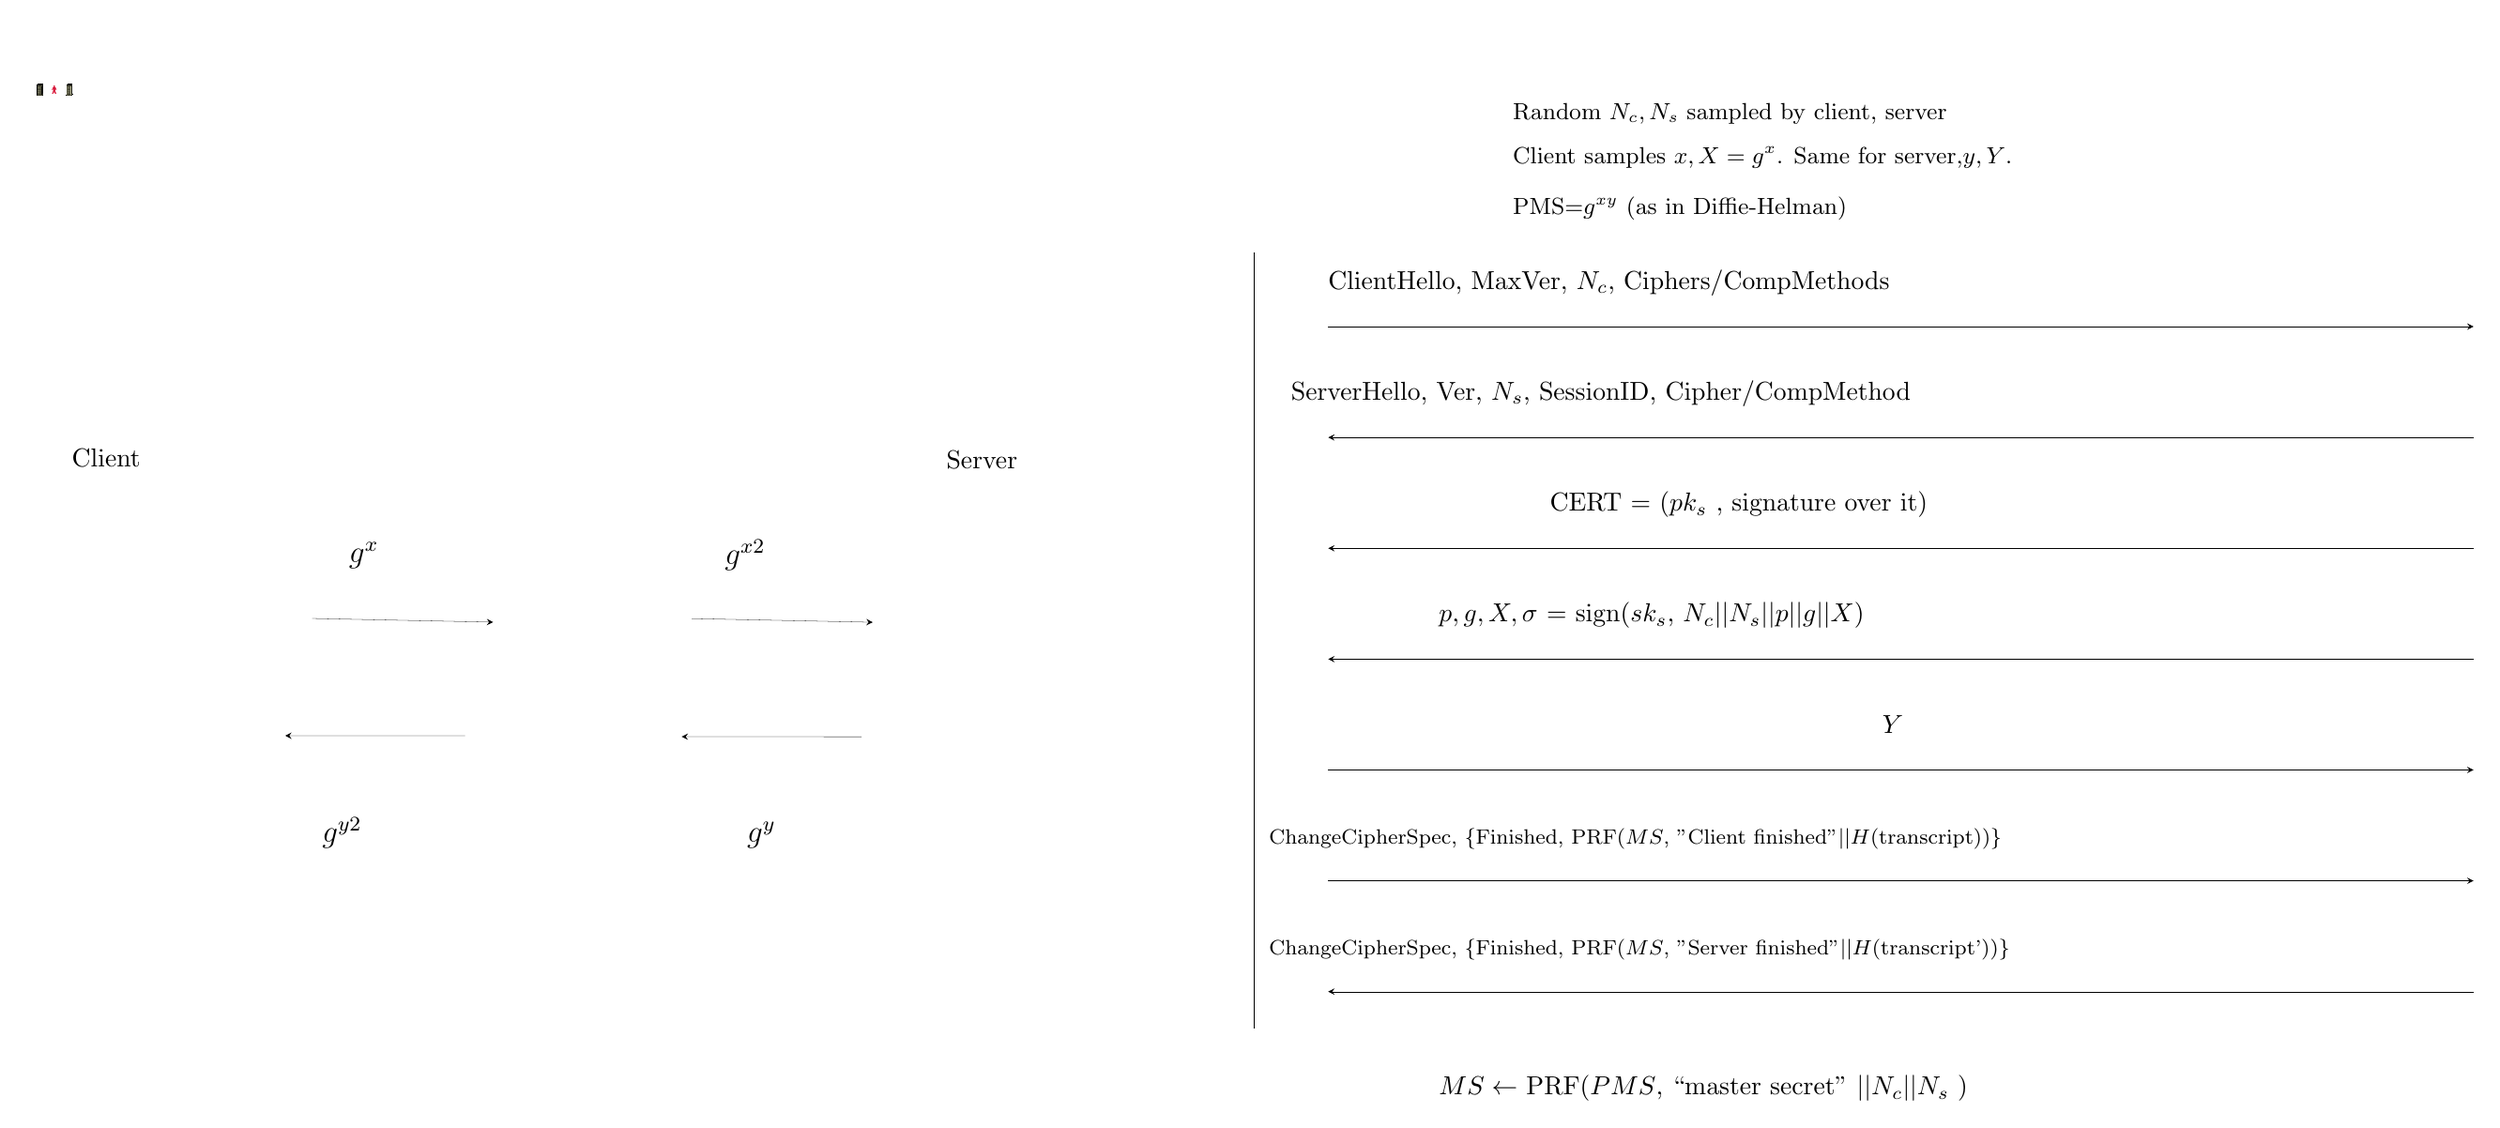
\begin{tikzpicture}[even odd rule]
\pgftransformxscale{1.000000}
\pgftransformyscale{-1.000000}
\definecolor{dialinecolor}{rgb}{0.000000, 0.000000, 0.000000}
\pgfsetstrokecolor{dialinecolor}
\pgfsetstrokeopacity{1.000000}
\definecolor{diafillcolor}{rgb}{1.000000, 1.000000, 1.000000}
\pgfsetfillcolor{diafillcolor}
\pgfsetfillopacity{1.000000}
\pgfsetlinewidth{0.100000\du}
\pgfsetdash{}{0pt}
\pgfsetbuttcap
\pgfsetmiterjoin
\pgfsetlinewidth{0.000000\du}
\pgfsetbuttcap
\pgfsetmiterjoin
\pgfsetdash{}{0pt}
\definecolor{diafillcolor}{rgb}{0.717647, 0.717647, 0.588235}
\pgfsetfillcolor{diafillcolor}
\pgfsetfillopacity{1.000000}
\definecolor{dialinecolor}{rgb}{0.000000, 0.000000, 0.000000}
\pgfsetstrokecolor{dialinecolor}
\pgfsetstrokeopacity{1.000000}
\pgfpathmoveto{\pgfpoint{12.223441\du}{10.404378\du}}
\pgfpathlineto{\pgfpoint{14.033748\du}{10.404378\du}}
\pgfpathlineto{\pgfpoint{14.033748\du}{6.543804\du}}
\pgfpathlineto{\pgfpoint{12.223441\du}{6.543804\du}}
\pgfpathlineto{\pgfpoint{12.223441\du}{10.404378\du}}
\pgfpathclose
\pgfusepath{fill,stroke}
\pgfsetlinewidth{0.010000\du}
\pgfsetmiterjoin
\pgfsetdash{}{0pt}
\definecolor{dialinecolor}{rgb}{0.286275, 0.286275, 0.211765}
\pgfsetstrokecolor{dialinecolor}
\pgfsetstrokeopacity{1.000000}
\pgfpathmoveto{\pgfpoint{12.223441\du}{10.404378\du}}
\pgfpathlineto{\pgfpoint{14.033748\du}{10.404378\du}}
\pgfpathlineto{\pgfpoint{14.033748\du}{6.543804\du}}
\pgfpathlineto{\pgfpoint{12.223441\du}{6.543804\du}}
\pgfpathlineto{\pgfpoint{12.223441\du}{10.404378\du}}
\pgfusepath{stroke}
\pgfsetlinewidth{0.000000\du}
\pgfsetbuttcap
\pgfsetmiterjoin
\pgfsetdash{}{0pt}
\definecolor{diafillcolor}{rgb}{0.788235, 0.788235, 0.713726}
\pgfsetfillcolor{diafillcolor}
\pgfsetfillopacity{1.000000}
\definecolor{dialinecolor}{rgb}{0.000000, 0.000000, 0.000000}
\pgfsetstrokecolor{dialinecolor}
\pgfsetstrokeopacity{1.000000}
\pgfpathmoveto{\pgfpoint{12.223441\du}{6.543817\du}}
\pgfpathlineto{\pgfpoint{12.569312\du}{6.200121\du}}
\pgfpathlineto{\pgfpoint{14.314749\du}{6.200121\du}}
\pgfpathlineto{\pgfpoint{14.033796\du}{6.543817\du}}
\pgfpathlineto{\pgfpoint{12.223441\du}{6.543817\du}}
\pgfpathclose
\pgfusepath{fill,stroke}
\pgfsetlinewidth{0.010000\du}
\pgfsetmiterjoin
\pgfsetdash{}{0pt}
\definecolor{dialinecolor}{rgb}{0.286275, 0.286275, 0.211765}
\pgfsetstrokecolor{dialinecolor}
\pgfsetstrokeopacity{1.000000}
\pgfpathmoveto{\pgfpoint{12.223441\du}{6.543817\du}}
\pgfpathlineto{\pgfpoint{12.569312\du}{6.200121\du}}
\pgfpathlineto{\pgfpoint{14.314749\du}{6.200121\du}}
\pgfpathlineto{\pgfpoint{14.033796\du}{6.543817\du}}
\pgfpathlineto{\pgfpoint{12.223441\du}{6.543817\du}}
\pgfusepath{stroke}
\pgfsetlinewidth{0.000000\du}
\pgfsetbuttcap
\pgfsetmiterjoin
\pgfsetdash{}{0pt}
\definecolor{diafillcolor}{rgb}{0.478431, 0.478431, 0.352941}
\pgfsetfillcolor{diafillcolor}
\pgfsetfillopacity{1.000000}
\definecolor{dialinecolor}{rgb}{0.000000, 0.000000, 0.000000}
\pgfsetstrokecolor{dialinecolor}
\pgfsetstrokeopacity{1.000000}
\pgfpathmoveto{\pgfpoint{14.033676\du}{10.404378\du}}
\pgfpathlineto{\pgfpoint{14.314628\du}{9.869190\du}}
\pgfpathlineto{\pgfpoint{14.314628\du}{6.200000\du}}
\pgfpathlineto{\pgfpoint{14.033676\du}{6.543696\du}}
\pgfpathlineto{\pgfpoint{14.033676\du}{10.404257\du}}
\pgfpathlineto{\pgfpoint{14.033676\du}{10.404378\du}}
\pgfpathclose
\pgfusepath{fill,stroke}
\pgfsetlinewidth{0.010000\du}
\pgfsetmiterjoin
\pgfsetdash{}{0pt}
\definecolor{dialinecolor}{rgb}{0.286275, 0.286275, 0.211765}
\pgfsetstrokecolor{dialinecolor}
\pgfsetstrokeopacity{1.000000}
\pgfpathmoveto{\pgfpoint{14.033676\du}{10.404378\du}}
\pgfpathlineto{\pgfpoint{14.314628\du}{9.869190\du}}
\pgfpathlineto{\pgfpoint{14.314628\du}{6.200000\du}}
\pgfpathlineto{\pgfpoint{14.033676\du}{6.543696\du}}
\pgfpathlineto{\pgfpoint{14.033676\du}{10.404257\du}}
\pgfusepath{stroke}
\pgfsetlinewidth{0.000000\du}
\pgfsetbuttcap
\pgfsetmiterjoin
\pgfsetdash{}{0pt}
\definecolor{diafillcolor}{rgb}{0.717647, 0.717647, 0.588235}
\pgfsetfillcolor{diafillcolor}
\pgfsetfillopacity{1.000000}
\definecolor{dialinecolor}{rgb}{0.000000, 0.000000, 0.000000}
\pgfsetstrokecolor{dialinecolor}
\pgfsetstrokeopacity{1.000000}
\pgfpathmoveto{\pgfpoint{14.177779\du}{10.576770\du}}
\pgfpathlineto{\pgfpoint{14.033796\du}{10.404378\du}}
\pgfpathlineto{\pgfpoint{12.223441\du}{10.404378\du}}
\pgfpathlineto{\pgfpoint{12.049840\du}{10.576770\du}}
\pgfpathlineto{\pgfpoint{14.177779\du}{10.576770\du}}
\pgfpathlineto{\pgfpoint{14.177779\du}{10.576770\du}}
\pgfpathclose
\pgfusepath{fill,stroke}
\pgfsetlinewidth{0.010000\du}
\pgfsetmiterjoin
\pgfsetdash{}{0pt}
\definecolor{dialinecolor}{rgb}{0.286275, 0.286275, 0.211765}
\pgfsetstrokecolor{dialinecolor}
\pgfsetstrokeopacity{1.000000}
\pgfpathmoveto{\pgfpoint{14.177779\du}{10.576770\du}}
\pgfpathlineto{\pgfpoint{14.033796\du}{10.404378\du}}
\pgfpathlineto{\pgfpoint{12.223441\du}{10.404378\du}}
\pgfpathlineto{\pgfpoint{12.049840\du}{10.576770\du}}
\pgfpathlineto{\pgfpoint{14.177779\du}{10.576770\du}}
\pgfusepath{stroke}
\pgfsetlinewidth{0.000000\du}
\pgfsetbuttcap
\pgfsetmiterjoin
\pgfsetdash{}{0pt}
\definecolor{diafillcolor}{rgb}{0.717647, 0.717647, 0.588235}
\pgfsetfillcolor{diafillcolor}
\pgfsetfillopacity{1.000000}
\definecolor{dialinecolor}{rgb}{0.000000, 0.000000, 0.000000}
\pgfsetstrokecolor{dialinecolor}
\pgfsetstrokeopacity{1.000000}
\pgfpathmoveto{\pgfpoint{14.177779\du}{10.576770\du}}
\pgfpathlineto{\pgfpoint{14.457764\du}{9.977871\du}}
\pgfpathlineto{\pgfpoint{14.314628\du}{9.869190\du}}
\pgfpathlineto{\pgfpoint{14.033676\du}{10.404378\du}}
\pgfpathlineto{\pgfpoint{14.177658\du}{10.576770\du}}
\pgfpathlineto{\pgfpoint{14.177779\du}{10.576770\du}}
\pgfpathclose
\pgfusepath{fill,stroke}
\pgfsetlinewidth{0.010000\du}
\pgfsetmiterjoin
\pgfsetdash{}{0pt}
\definecolor{dialinecolor}{rgb}{0.286275, 0.286275, 0.211765}
\pgfsetstrokecolor{dialinecolor}
\pgfsetstrokeopacity{1.000000}
\pgfpathmoveto{\pgfpoint{14.177779\du}{10.576770\du}}
\pgfpathlineto{\pgfpoint{14.457764\du}{9.977871\du}}
\pgfpathlineto{\pgfpoint{14.314628\du}{9.869190\du}}
\pgfpathlineto{\pgfpoint{14.033676\du}{10.404378\du}}
\pgfpathlineto{\pgfpoint{14.177658\du}{10.576770\du}}
\pgfusepath{stroke}
\pgfsetlinewidth{0.000000\du}
\pgfsetbuttcap
\pgfsetmiterjoin
\pgfsetdash{}{0pt}
\definecolor{diafillcolor}{rgb}{0.717647, 0.717647, 0.588235}
\pgfsetfillcolor{diafillcolor}
\pgfsetfillopacity{1.000000}
\pgfpathmoveto{\pgfpoint{14.033676\du}{10.404378\du}}
\pgfpathlineto{\pgfpoint{12.223320\du}{10.404378\du}}
\pgfpathlineto{\pgfpoint{14.033676\du}{10.404378\du}}
\pgfpathclose
\pgfusepath{fill}
\pgfsetlinewidth{0.010000\du}
\pgfsetmiterjoin
\pgfsetdash{}{0pt}
\definecolor{dialinecolor}{rgb}{0.286275, 0.286275, 0.211765}
\pgfsetstrokecolor{dialinecolor}
\pgfsetstrokeopacity{1.000000}
\pgfpathmoveto{\pgfpoint{14.033676\du}{10.404378\du}}
\pgfpathlineto{\pgfpoint{12.223320\du}{10.404378\du}}
\pgfusepath{stroke}
\pgfsetlinewidth{0.000000\du}
\pgfsetbuttcap
\pgfsetmiterjoin
\pgfsetdash{}{0pt}
\definecolor{diafillcolor}{rgb}{0.717647, 0.717647, 0.588235}
\pgfsetfillcolor{diafillcolor}
\pgfsetfillopacity{1.000000}
\pgfpathmoveto{\pgfpoint{14.314628\du}{9.869190\du}}
\pgfpathlineto{\pgfpoint{14.033676\du}{10.404378\du}}
\pgfpathlineto{\pgfpoint{14.314628\du}{9.869190\du}}
\pgfpathclose
\pgfusepath{fill}
\pgfsetlinewidth{0.010000\du}
\pgfsetmiterjoin
\pgfsetdash{}{0pt}
\definecolor{dialinecolor}{rgb}{0.286275, 0.286275, 0.211765}
\pgfsetstrokecolor{dialinecolor}
\pgfsetstrokeopacity{1.000000}
\pgfpathmoveto{\pgfpoint{14.314628\du}{9.869190\du}}
\pgfpathlineto{\pgfpoint{14.033676\du}{10.404378\du}}
\pgfusepath{stroke}
\pgfsetlinewidth{0.000000\du}
\pgfsetbuttcap
\pgfsetmiterjoin
\pgfsetdash{}{0pt}
\definecolor{diafillcolor}{rgb}{0.717647, 0.717647, 0.588235}
\pgfsetfillcolor{diafillcolor}
\pgfsetfillopacity{1.000000}
\pgfpathmoveto{\pgfpoint{12.224287\du}{6.721890\du}}
\pgfpathlineto{\pgfpoint{14.026543\du}{6.721890\du}}
\pgfpathlineto{\pgfpoint{12.224287\du}{6.721890\du}}
\pgfpathclose
\pgfusepath{fill}
\pgfsetlinewidth{0.010000\du}
\pgfsetmiterjoin
\pgfsetdash{}{0pt}
\definecolor{dialinecolor}{rgb}{0.286275, 0.286275, 0.211765}
\pgfsetstrokecolor{dialinecolor}
\pgfsetstrokeopacity{1.000000}
\pgfpathmoveto{\pgfpoint{12.224287\du}{6.721890\du}}
\pgfpathlineto{\pgfpoint{14.026543\du}{6.721890\du}}
\pgfusepath{stroke}
\pgfsetlinewidth{0.000000\du}
\pgfsetbuttcap
\pgfsetmiterjoin
\pgfsetdash{}{0pt}
\definecolor{diafillcolor}{rgb}{0.717647, 0.717647, 0.588235}
\pgfsetfillcolor{diafillcolor}
\pgfsetfillopacity{1.000000}
\pgfpathmoveto{\pgfpoint{12.222715\du}{6.743772\du}}
\pgfpathlineto{\pgfpoint{14.024971\du}{6.743772\du}}
\pgfpathlineto{\pgfpoint{12.222715\du}{6.743772\du}}
\pgfpathclose
\pgfusepath{fill}
\pgfsetlinewidth{0.010000\du}
\pgfsetmiterjoin
\pgfsetdash{}{0pt}
\definecolor{dialinecolor}{rgb}{0.286275, 0.286275, 0.211765}
\pgfsetstrokecolor{dialinecolor}
\pgfsetstrokeopacity{1.000000}
\pgfpathmoveto{\pgfpoint{12.222715\du}{6.743772\du}}
\pgfpathlineto{\pgfpoint{14.024971\du}{6.743772\du}}
\pgfusepath{stroke}
\pgfsetlinewidth{0.000000\du}
\pgfsetbuttcap
\pgfsetmiterjoin
\pgfsetdash{}{0pt}
\definecolor{diafillcolor}{rgb}{0.717647, 0.717647, 0.588235}
\pgfsetfillcolor{diafillcolor}
\pgfsetfillopacity{1.000000}
\pgfpathmoveto{\pgfpoint{13.658548\du}{7.205820\du}}
\pgfpathlineto{\pgfpoint{12.345058\du}{7.205820\du}}
\pgfpathlineto{\pgfpoint{12.345058\du}{7.326712\du}}
\pgfpathlineto{\pgfpoint{12.587809\du}{7.326712\du}}
\pgfpathlineto{\pgfpoint{13.658548\du}{7.205820\du}}
\pgfpathclose
\pgfusepath{fill}
\pgfsetlinewidth{0.010000\du}
\pgfsetmiterjoin
\pgfsetdash{}{0pt}
\definecolor{dialinecolor}{rgb}{0.286275, 0.286275, 0.211765}
\pgfsetstrokecolor{dialinecolor}
\pgfsetstrokeopacity{1.000000}
\pgfpathmoveto{\pgfpoint{13.658548\du}{7.205820\du}}
\pgfpathlineto{\pgfpoint{12.345058\du}{7.205820\du}}
\pgfpathlineto{\pgfpoint{12.345058\du}{7.326712\du}}
\pgfpathlineto{\pgfpoint{12.587809\du}{7.326712\du}}
\pgfusepath{stroke}
\pgfsetlinewidth{0.000000\du}
\pgfsetbuttcap
\pgfsetmiterjoin
\pgfsetdash{}{0pt}
\definecolor{diafillcolor}{rgb}{0.717647, 0.717647, 0.588235}
\pgfsetfillcolor{diafillcolor}
\pgfsetfillopacity{1.000000}
\pgfpathmoveto{\pgfpoint{13.658548\du}{7.429954\du}}
\pgfpathlineto{\pgfpoint{12.345058\du}{7.429954\du}}
\pgfpathlineto{\pgfpoint{12.345058\du}{7.550846\du}}
\pgfpathlineto{\pgfpoint{12.587809\du}{7.550846\du}}
\pgfpathlineto{\pgfpoint{13.658548\du}{7.429954\du}}
\pgfpathclose
\pgfusepath{fill}
\pgfsetlinewidth{0.010000\du}
\pgfsetmiterjoin
\pgfsetdash{}{0pt}
\definecolor{dialinecolor}{rgb}{0.286275, 0.286275, 0.211765}
\pgfsetstrokecolor{dialinecolor}
\pgfsetstrokeopacity{1.000000}
\pgfpathmoveto{\pgfpoint{13.658548\du}{7.429954\du}}
\pgfpathlineto{\pgfpoint{12.345058\du}{7.429954\du}}
\pgfpathlineto{\pgfpoint{12.345058\du}{7.550846\du}}
\pgfpathlineto{\pgfpoint{12.587809\du}{7.550846\du}}
\pgfusepath{stroke}
\pgfsetlinewidth{0.000000\du}
\pgfsetbuttcap
\pgfsetmiterjoin
\pgfsetdash{}{0pt}
\definecolor{diafillcolor}{rgb}{0.717647, 0.717647, 0.588235}
\pgfsetfillcolor{diafillcolor}
\pgfsetfillopacity{1.000000}
\pgfpathmoveto{\pgfpoint{13.658548\du}{7.654208\du}}
\pgfpathlineto{\pgfpoint{12.345058\du}{7.654208\du}}
\pgfpathlineto{\pgfpoint{12.345058\du}{7.775100\du}}
\pgfpathlineto{\pgfpoint{12.587809\du}{7.775100\du}}
\pgfpathlineto{\pgfpoint{13.658548\du}{7.654208\du}}
\pgfpathclose
\pgfusepath{fill}
\pgfsetlinewidth{0.010000\du}
\pgfsetmiterjoin
\pgfsetdash{}{0pt}
\definecolor{dialinecolor}{rgb}{0.286275, 0.286275, 0.211765}
\pgfsetstrokecolor{dialinecolor}
\pgfsetstrokeopacity{1.000000}
\pgfpathmoveto{\pgfpoint{13.658548\du}{7.654208\du}}
\pgfpathlineto{\pgfpoint{12.345058\du}{7.654208\du}}
\pgfpathlineto{\pgfpoint{12.345058\du}{7.775100\du}}
\pgfpathlineto{\pgfpoint{12.587809\du}{7.775100\du}}
\pgfusepath{stroke}
\pgfsetlinewidth{0.000000\du}
\pgfsetbuttcap
\pgfsetmiterjoin
\pgfsetdash{}{0pt}
\definecolor{diafillcolor}{rgb}{0.717647, 0.717647, 0.588235}
\pgfsetfillcolor{diafillcolor}
\pgfsetfillopacity{1.000000}
\pgfpathmoveto{\pgfpoint{13.658548\du}{7.878342\du}}
\pgfpathlineto{\pgfpoint{12.345058\du}{7.878342\du}}
\pgfpathlineto{\pgfpoint{12.345058\du}{7.999234\du}}
\pgfpathlineto{\pgfpoint{12.587809\du}{7.999234\du}}
\pgfpathlineto{\pgfpoint{13.658548\du}{7.878342\du}}
\pgfpathclose
\pgfusepath{fill}
\pgfsetlinewidth{0.010000\du}
\pgfsetmiterjoin
\pgfsetdash{}{0pt}
\definecolor{dialinecolor}{rgb}{0.286275, 0.286275, 0.211765}
\pgfsetstrokecolor{dialinecolor}
\pgfsetstrokeopacity{1.000000}
\pgfpathmoveto{\pgfpoint{13.658548\du}{7.878342\du}}
\pgfpathlineto{\pgfpoint{12.345058\du}{7.878342\du}}
\pgfpathlineto{\pgfpoint{12.345058\du}{7.999234\du}}
\pgfpathlineto{\pgfpoint{12.587809\du}{7.999234\du}}
\pgfusepath{stroke}
\pgfsetlinewidth{0.000000\du}
\pgfsetbuttcap
\pgfsetmiterjoin
\pgfsetdash{}{0pt}
\definecolor{diafillcolor}{rgb}{0.717647, 0.717647, 0.588235}
\pgfsetfillcolor{diafillcolor}
\pgfsetfillopacity{1.000000}
\pgfpathmoveto{\pgfpoint{13.658548\du}{8.102596\du}}
\pgfpathlineto{\pgfpoint{12.345058\du}{8.102596\du}}
\pgfpathlineto{\pgfpoint{12.345058\du}{8.223488\du}}
\pgfpathlineto{\pgfpoint{12.587809\du}{8.223488\du}}
\pgfpathlineto{\pgfpoint{13.658548\du}{8.102596\du}}
\pgfpathclose
\pgfusepath{fill}
\pgfsetlinewidth{0.010000\du}
\pgfsetmiterjoin
\pgfsetdash{}{0pt}
\definecolor{dialinecolor}{rgb}{0.286275, 0.286275, 0.211765}
\pgfsetstrokecolor{dialinecolor}
\pgfsetstrokeopacity{1.000000}
\pgfpathmoveto{\pgfpoint{13.658548\du}{8.102596\du}}
\pgfpathlineto{\pgfpoint{12.345058\du}{8.102596\du}}
\pgfpathlineto{\pgfpoint{12.345058\du}{8.223488\du}}
\pgfpathlineto{\pgfpoint{12.587809\du}{8.223488\du}}
\pgfusepath{stroke}
\pgfsetlinewidth{0.000000\du}
\pgfsetbuttcap
\pgfsetmiterjoin
\pgfsetdash{}{0pt}
\definecolor{diafillcolor}{rgb}{0.717647, 0.717647, 0.588235}
\pgfsetfillcolor{diafillcolor}
\pgfsetfillopacity{1.000000}
\pgfpathmoveto{\pgfpoint{13.658548\du}{8.326730\du}}
\pgfpathlineto{\pgfpoint{12.345058\du}{8.326730\du}}
\pgfpathlineto{\pgfpoint{12.345058\du}{8.447622\du}}
\pgfpathlineto{\pgfpoint{12.587809\du}{8.447622\du}}
\pgfpathlineto{\pgfpoint{13.658548\du}{8.326730\du}}
\pgfpathclose
\pgfusepath{fill}
\pgfsetlinewidth{0.010000\du}
\pgfsetmiterjoin
\pgfsetdash{}{0pt}
\definecolor{dialinecolor}{rgb}{0.286275, 0.286275, 0.211765}
\pgfsetstrokecolor{dialinecolor}
\pgfsetstrokeopacity{1.000000}
\pgfpathmoveto{\pgfpoint{13.658548\du}{8.326730\du}}
\pgfpathlineto{\pgfpoint{12.345058\du}{8.326730\du}}
\pgfpathlineto{\pgfpoint{12.345058\du}{8.447622\du}}
\pgfpathlineto{\pgfpoint{12.587809\du}{8.447622\du}}
\pgfusepath{stroke}
\pgfsetlinewidth{0.000000\du}
\pgfsetbuttcap
\pgfsetmiterjoin
\pgfsetdash{}{0pt}
\definecolor{diafillcolor}{rgb}{0.717647, 0.717647, 0.588235}
\pgfsetfillcolor{diafillcolor}
\pgfsetfillopacity{1.000000}
\pgfpathmoveto{\pgfpoint{13.658548\du}{8.550864\du}}
\pgfpathlineto{\pgfpoint{12.345058\du}{8.550864\du}}
\pgfpathlineto{\pgfpoint{12.345058\du}{8.671755\du}}
\pgfpathlineto{\pgfpoint{12.587809\du}{8.671755\du}}
\pgfpathlineto{\pgfpoint{13.658548\du}{8.550864\du}}
\pgfpathclose
\pgfusepath{fill}
\pgfsetlinewidth{0.010000\du}
\pgfsetmiterjoin
\pgfsetdash{}{0pt}
\definecolor{dialinecolor}{rgb}{0.286275, 0.286275, 0.211765}
\pgfsetstrokecolor{dialinecolor}
\pgfsetstrokeopacity{1.000000}
\pgfpathmoveto{\pgfpoint{13.658548\du}{8.550864\du}}
\pgfpathlineto{\pgfpoint{12.345058\du}{8.550864\du}}
\pgfpathlineto{\pgfpoint{12.345058\du}{8.671755\du}}
\pgfpathlineto{\pgfpoint{12.587809\du}{8.671755\du}}
\pgfusepath{stroke}
\pgfsetlinewidth{0.000000\du}
\pgfsetbuttcap
\pgfsetmiterjoin
\pgfsetdash{}{0pt}
\definecolor{diafillcolor}{rgb}{0.717647, 0.717647, 0.588235}
\pgfsetfillcolor{diafillcolor}
\pgfsetfillopacity{1.000000}
\pgfpathmoveto{\pgfpoint{13.658548\du}{8.775118\du}}
\pgfpathlineto{\pgfpoint{12.345058\du}{8.775118\du}}
\pgfpathlineto{\pgfpoint{12.345058\du}{8.896010\du}}
\pgfpathlineto{\pgfpoint{12.587809\du}{8.896010\du}}
\pgfpathlineto{\pgfpoint{13.658548\du}{8.775118\du}}
\pgfpathclose
\pgfusepath{fill}
\pgfsetlinewidth{0.010000\du}
\pgfsetmiterjoin
\pgfsetdash{}{0pt}
\definecolor{dialinecolor}{rgb}{0.286275, 0.286275, 0.211765}
\pgfsetstrokecolor{dialinecolor}
\pgfsetstrokeopacity{1.000000}
\pgfpathmoveto{\pgfpoint{13.658548\du}{8.775118\du}}
\pgfpathlineto{\pgfpoint{12.345058\du}{8.775118\du}}
\pgfpathlineto{\pgfpoint{12.345058\du}{8.896010\du}}
\pgfpathlineto{\pgfpoint{12.587809\du}{8.896010\du}}
\pgfusepath{stroke}
\pgfsetlinewidth{0.000000\du}
\pgfsetbuttcap
\pgfsetmiterjoin
\pgfsetdash{}{0pt}
\definecolor{diafillcolor}{rgb}{0.717647, 0.717647, 0.588235}
\pgfsetfillcolor{diafillcolor}
\pgfsetfillopacity{1.000000}
\pgfpathmoveto{\pgfpoint{13.658548\du}{8.999252\du}}
\pgfpathlineto{\pgfpoint{12.345058\du}{8.999252\du}}
\pgfpathlineto{\pgfpoint{12.345058\du}{9.120143\du}}
\pgfpathlineto{\pgfpoint{12.587809\du}{9.120143\du}}
\pgfpathlineto{\pgfpoint{13.658548\du}{8.999252\du}}
\pgfpathclose
\pgfusepath{fill}
\pgfsetlinewidth{0.010000\du}
\pgfsetmiterjoin
\pgfsetdash{}{0pt}
\definecolor{dialinecolor}{rgb}{0.286275, 0.286275, 0.211765}
\pgfsetstrokecolor{dialinecolor}
\pgfsetstrokeopacity{1.000000}
\pgfpathmoveto{\pgfpoint{13.658548\du}{8.999252\du}}
\pgfpathlineto{\pgfpoint{12.345058\du}{8.999252\du}}
\pgfpathlineto{\pgfpoint{12.345058\du}{9.120143\du}}
\pgfpathlineto{\pgfpoint{12.587809\du}{9.120143\du}}
\pgfusepath{stroke}
\pgfsetlinewidth{0.000000\du}
\pgfsetbuttcap
\pgfsetmiterjoin
\pgfsetdash{}{0pt}
\definecolor{diafillcolor}{rgb}{0.717647, 0.717647, 0.588235}
\pgfsetfillcolor{diafillcolor}
\pgfsetfillopacity{1.000000}
\pgfpathmoveto{\pgfpoint{13.658548\du}{9.223506\du}}
\pgfpathlineto{\pgfpoint{12.345058\du}{9.223506\du}}
\pgfpathlineto{\pgfpoint{12.345058\du}{9.344398\du}}
\pgfpathlineto{\pgfpoint{12.587809\du}{9.344398\du}}
\pgfpathlineto{\pgfpoint{13.658548\du}{9.223506\du}}
\pgfpathclose
\pgfusepath{fill}
\pgfsetlinewidth{0.010000\du}
\pgfsetmiterjoin
\pgfsetdash{}{0pt}
\definecolor{dialinecolor}{rgb}{0.286275, 0.286275, 0.211765}
\pgfsetstrokecolor{dialinecolor}
\pgfsetstrokeopacity{1.000000}
\pgfpathmoveto{\pgfpoint{13.658548\du}{9.223506\du}}
\pgfpathlineto{\pgfpoint{12.345058\du}{9.223506\du}}
\pgfpathlineto{\pgfpoint{12.345058\du}{9.344398\du}}
\pgfpathlineto{\pgfpoint{12.587809\du}{9.344398\du}}
\pgfusepath{stroke}
\pgfsetlinewidth{0.000000\du}
\pgfsetbuttcap
\pgfsetmiterjoin
\pgfsetdash{}{0pt}
\definecolor{diafillcolor}{rgb}{0.717647, 0.717647, 0.588235}
\pgfsetfillcolor{diafillcolor}
\pgfsetfillopacity{1.000000}
\pgfpathmoveto{\pgfpoint{13.658548\du}{9.447640\du}}
\pgfpathlineto{\pgfpoint{12.345058\du}{9.447640\du}}
\pgfpathlineto{\pgfpoint{12.345058\du}{9.568531\du}}
\pgfpathlineto{\pgfpoint{12.587809\du}{9.568531\du}}
\pgfpathlineto{\pgfpoint{13.658548\du}{9.447640\du}}
\pgfpathclose
\pgfusepath{fill}
\pgfsetlinewidth{0.010000\du}
\pgfsetmiterjoin
\pgfsetdash{}{0pt}
\definecolor{dialinecolor}{rgb}{0.286275, 0.286275, 0.211765}
\pgfsetstrokecolor{dialinecolor}
\pgfsetstrokeopacity{1.000000}
\pgfpathmoveto{\pgfpoint{13.658548\du}{9.447640\du}}
\pgfpathlineto{\pgfpoint{12.345058\du}{9.447640\du}}
\pgfpathlineto{\pgfpoint{12.345058\du}{9.568531\du}}
\pgfpathlineto{\pgfpoint{12.587809\du}{9.568531\du}}
\pgfusepath{stroke}
\pgfsetlinewidth{0.000000\du}
\pgfsetbuttcap
\pgfsetmiterjoin
\pgfsetdash{}{0pt}
\definecolor{diafillcolor}{rgb}{0.717647, 0.717647, 0.588235}
\pgfsetfillcolor{diafillcolor}
\pgfsetfillopacity{1.000000}
\pgfpathmoveto{\pgfpoint{13.658548\du}{9.671773\du}}
\pgfpathlineto{\pgfpoint{12.345058\du}{9.671773\du}}
\pgfpathlineto{\pgfpoint{12.345058\du}{9.792665\du}}
\pgfpathlineto{\pgfpoint{12.587809\du}{9.792665\du}}
\pgfpathlineto{\pgfpoint{13.658548\du}{9.671773\du}}
\pgfpathclose
\pgfusepath{fill}
\pgfsetlinewidth{0.010000\du}
\pgfsetmiterjoin
\pgfsetdash{}{0pt}
\definecolor{dialinecolor}{rgb}{0.286275, 0.286275, 0.211765}
\pgfsetstrokecolor{dialinecolor}
\pgfsetstrokeopacity{1.000000}
\pgfpathmoveto{\pgfpoint{13.658548\du}{9.671773\du}}
\pgfpathlineto{\pgfpoint{12.345058\du}{9.671773\du}}
\pgfpathlineto{\pgfpoint{12.345058\du}{9.792665\du}}
\pgfpathlineto{\pgfpoint{12.587809\du}{9.792665\du}}
\pgfusepath{stroke}
\pgfsetlinewidth{0.000000\du}
\pgfsetbuttcap
\pgfsetmiterjoin
\pgfsetdash{}{0pt}
\definecolor{diafillcolor}{rgb}{0.717647, 0.717647, 0.588235}
\pgfsetfillcolor{diafillcolor}
\pgfsetfillopacity{1.000000}
\pgfpathmoveto{\pgfpoint{13.658548\du}{9.896028\du}}
\pgfpathlineto{\pgfpoint{12.345058\du}{9.896028\du}}
\pgfpathlineto{\pgfpoint{12.345058\du}{10.016919\du}}
\pgfpathlineto{\pgfpoint{12.587809\du}{10.016919\du}}
\pgfpathlineto{\pgfpoint{13.658548\du}{9.896028\du}}
\pgfpathclose
\pgfusepath{fill}
\pgfsetlinewidth{0.010000\du}
\pgfsetmiterjoin
\pgfsetdash{}{0pt}
\definecolor{dialinecolor}{rgb}{0.286275, 0.286275, 0.211765}
\pgfsetstrokecolor{dialinecolor}
\pgfsetstrokeopacity{1.000000}
\pgfpathmoveto{\pgfpoint{13.658548\du}{9.896028\du}}
\pgfpathlineto{\pgfpoint{12.345058\du}{9.896028\du}}
\pgfpathlineto{\pgfpoint{12.345058\du}{10.016919\du}}
\pgfpathlineto{\pgfpoint{12.587809\du}{10.016919\du}}
\pgfusepath{stroke}
\pgfsetlinewidth{0.000000\du}
\pgfsetbuttcap
\pgfsetmiterjoin
\pgfsetdash{}{0pt}
\definecolor{diafillcolor}{rgb}{0.717647, 0.717647, 0.588235}
\pgfsetfillcolor{diafillcolor}
\pgfsetfillopacity{1.000000}
\pgfpathmoveto{\pgfpoint{13.658548\du}{10.120161\du}}
\pgfpathlineto{\pgfpoint{12.345058\du}{10.120161\du}}
\pgfpathlineto{\pgfpoint{12.345058\du}{10.241053\du}}
\pgfpathlineto{\pgfpoint{12.587809\du}{10.241053\du}}
\pgfpathlineto{\pgfpoint{13.658548\du}{10.120161\du}}
\pgfpathclose
\pgfusepath{fill}
\pgfsetlinewidth{0.010000\du}
\pgfsetmiterjoin
\pgfsetdash{}{0pt}
\definecolor{dialinecolor}{rgb}{0.286275, 0.286275, 0.211765}
\pgfsetstrokecolor{dialinecolor}
\pgfsetstrokeopacity{1.000000}
\pgfpathmoveto{\pgfpoint{13.658548\du}{10.120161\du}}
\pgfpathlineto{\pgfpoint{12.345058\du}{10.120161\du}}
\pgfpathlineto{\pgfpoint{12.345058\du}{10.241053\du}}
\pgfpathlineto{\pgfpoint{12.587809\du}{10.241053\du}}
\pgfusepath{stroke}
\pgfsetlinewidth{0.100000\du}
\pgfsetdash{}{0pt}
\pgfsetbuttcap
\pgfsetmiterjoin
\pgfsetlinewidth{0.000000\du}
\pgfsetbuttcap
\pgfsetmiterjoin
\pgfsetdash{}{0pt}
\definecolor{diafillcolor}{rgb}{0.717647, 0.717647, 0.588235}
\pgfsetfillcolor{diafillcolor}
\pgfsetfillopacity{1.000000}
\definecolor{dialinecolor}{rgb}{0.000000, 0.000000, 0.000000}
\pgfsetstrokecolor{dialinecolor}
\pgfsetstrokeopacity{1.000000}
\pgfpathmoveto{\pgfpoint{0.871220\du}{10.409714\du}}
\pgfpathlineto{\pgfpoint{2.681528\du}{10.409714\du}}
\pgfpathlineto{\pgfpoint{2.681528\du}{6.549140\du}}
\pgfpathlineto{\pgfpoint{0.871220\du}{6.549140\du}}
\pgfpathlineto{\pgfpoint{0.871220\du}{10.409714\du}}
\pgfpathclose
\pgfusepath{fill,stroke}
\pgfsetlinewidth{0.010000\du}
\pgfsetmiterjoin
\pgfsetdash{}{0pt}
\definecolor{dialinecolor}{rgb}{0.286275, 0.286275, 0.211765}
\pgfsetstrokecolor{dialinecolor}
\pgfsetstrokeopacity{1.000000}
\pgfpathmoveto{\pgfpoint{0.871220\du}{10.409714\du}}
\pgfpathlineto{\pgfpoint{2.681528\du}{10.409714\du}}
\pgfpathlineto{\pgfpoint{2.681528\du}{6.549140\du}}
\pgfpathlineto{\pgfpoint{0.871220\du}{6.549140\du}}
\pgfpathlineto{\pgfpoint{0.871220\du}{10.409714\du}}
\pgfusepath{stroke}
\pgfsetlinewidth{0.000000\du}
\pgfsetbuttcap
\pgfsetmiterjoin
\pgfsetdash{}{0pt}
\definecolor{diafillcolor}{rgb}{0.788235, 0.788235, 0.713726}
\pgfsetfillcolor{diafillcolor}
\pgfsetfillopacity{1.000000}
\definecolor{dialinecolor}{rgb}{0.000000, 0.000000, 0.000000}
\pgfsetstrokecolor{dialinecolor}
\pgfsetstrokeopacity{1.000000}
\pgfpathmoveto{\pgfpoint{0.871220\du}{6.549152\du}}
\pgfpathlineto{\pgfpoint{1.217092\du}{6.205457\du}}
\pgfpathlineto{\pgfpoint{2.962529\du}{6.205457\du}}
\pgfpathlineto{\pgfpoint{2.681576\du}{6.549152\du}}
\pgfpathlineto{\pgfpoint{0.871220\du}{6.549152\du}}
\pgfpathclose
\pgfusepath{fill,stroke}
\pgfsetlinewidth{0.010000\du}
\pgfsetmiterjoin
\pgfsetdash{}{0pt}
\definecolor{dialinecolor}{rgb}{0.286275, 0.286275, 0.211765}
\pgfsetstrokecolor{dialinecolor}
\pgfsetstrokeopacity{1.000000}
\pgfpathmoveto{\pgfpoint{0.871220\du}{6.549152\du}}
\pgfpathlineto{\pgfpoint{1.217092\du}{6.205457\du}}
\pgfpathlineto{\pgfpoint{2.962529\du}{6.205457\du}}
\pgfpathlineto{\pgfpoint{2.681576\du}{6.549152\du}}
\pgfpathlineto{\pgfpoint{0.871220\du}{6.549152\du}}
\pgfusepath{stroke}
\pgfsetlinewidth{0.000000\du}
\pgfsetbuttcap
\pgfsetmiterjoin
\pgfsetdash{}{0pt}
\definecolor{diafillcolor}{rgb}{0.478431, 0.478431, 0.352941}
\pgfsetfillcolor{diafillcolor}
\pgfsetfillopacity{1.000000}
\definecolor{dialinecolor}{rgb}{0.000000, 0.000000, 0.000000}
\pgfsetstrokecolor{dialinecolor}
\pgfsetstrokeopacity{1.000000}
\pgfpathmoveto{\pgfpoint{2.681455\du}{10.409714\du}}
\pgfpathlineto{\pgfpoint{2.962408\du}{9.874525\du}}
\pgfpathlineto{\pgfpoint{2.962408\du}{6.205336\du}}
\pgfpathlineto{\pgfpoint{2.681455\du}{6.549031\du}}
\pgfpathlineto{\pgfpoint{2.681455\du}{10.409593\du}}
\pgfpathlineto{\pgfpoint{2.681455\du}{10.409714\du}}
\pgfpathclose
\pgfusepath{fill,stroke}
\pgfsetlinewidth{0.010000\du}
\pgfsetmiterjoin
\pgfsetdash{}{0pt}
\definecolor{dialinecolor}{rgb}{0.286275, 0.286275, 0.211765}
\pgfsetstrokecolor{dialinecolor}
\pgfsetstrokeopacity{1.000000}
\pgfpathmoveto{\pgfpoint{2.681455\du}{10.409714\du}}
\pgfpathlineto{\pgfpoint{2.962408\du}{9.874525\du}}
\pgfpathlineto{\pgfpoint{2.962408\du}{6.205336\du}}
\pgfpathlineto{\pgfpoint{2.681455\du}{6.549031\du}}
\pgfpathlineto{\pgfpoint{2.681455\du}{10.409593\du}}
\pgfusepath{stroke}
\pgfsetlinewidth{0.000000\du}
\pgfsetbuttcap
\pgfsetmiterjoin
\pgfsetdash{}{0pt}
\definecolor{diafillcolor}{rgb}{0.717647, 0.717647, 0.588235}
\pgfsetfillcolor{diafillcolor}
\pgfsetfillopacity{1.000000}
\definecolor{dialinecolor}{rgb}{0.000000, 0.000000, 0.000000}
\pgfsetstrokecolor{dialinecolor}
\pgfsetstrokeopacity{1.000000}
\pgfpathmoveto{\pgfpoint{2.825558\du}{10.582106\du}}
\pgfpathlineto{\pgfpoint{2.681576\du}{10.409714\du}}
\pgfpathlineto{\pgfpoint{0.871220\du}{10.409714\du}}
\pgfpathlineto{\pgfpoint{0.697619\du}{10.582106\du}}
\pgfpathlineto{\pgfpoint{2.825558\du}{10.582106\du}}
\pgfpathlineto{\pgfpoint{2.825558\du}{10.582106\du}}
\pgfpathclose
\pgfusepath{fill,stroke}
\pgfsetlinewidth{0.010000\du}
\pgfsetmiterjoin
\pgfsetdash{}{0pt}
\definecolor{dialinecolor}{rgb}{0.286275, 0.286275, 0.211765}
\pgfsetstrokecolor{dialinecolor}
\pgfsetstrokeopacity{1.000000}
\pgfpathmoveto{\pgfpoint{2.825558\du}{10.582106\du}}
\pgfpathlineto{\pgfpoint{2.681576\du}{10.409714\du}}
\pgfpathlineto{\pgfpoint{0.871220\du}{10.409714\du}}
\pgfpathlineto{\pgfpoint{0.697619\du}{10.582106\du}}
\pgfpathlineto{\pgfpoint{2.825558\du}{10.582106\du}}
\pgfusepath{stroke}
\pgfsetlinewidth{0.000000\du}
\pgfsetbuttcap
\pgfsetmiterjoin
\pgfsetdash{}{0pt}
\definecolor{diafillcolor}{rgb}{0.717647, 0.717647, 0.588235}
\pgfsetfillcolor{diafillcolor}
\pgfsetfillopacity{1.000000}
\definecolor{dialinecolor}{rgb}{0.000000, 0.000000, 0.000000}
\pgfsetstrokecolor{dialinecolor}
\pgfsetstrokeopacity{1.000000}
\pgfpathmoveto{\pgfpoint{2.825558\du}{10.582106\du}}
\pgfpathlineto{\pgfpoint{3.105544\du}{9.983207\du}}
\pgfpathlineto{\pgfpoint{2.962408\du}{9.874525\du}}
\pgfpathlineto{\pgfpoint{2.681455\du}{10.409714\du}}
\pgfpathlineto{\pgfpoint{2.825437\du}{10.582106\du}}
\pgfpathlineto{\pgfpoint{2.825558\du}{10.582106\du}}
\pgfpathclose
\pgfusepath{fill,stroke}
\pgfsetlinewidth{0.010000\du}
\pgfsetmiterjoin
\pgfsetdash{}{0pt}
\definecolor{dialinecolor}{rgb}{0.286275, 0.286275, 0.211765}
\pgfsetstrokecolor{dialinecolor}
\pgfsetstrokeopacity{1.000000}
\pgfpathmoveto{\pgfpoint{2.825558\du}{10.582106\du}}
\pgfpathlineto{\pgfpoint{3.105544\du}{9.983207\du}}
\pgfpathlineto{\pgfpoint{2.962408\du}{9.874525\du}}
\pgfpathlineto{\pgfpoint{2.681455\du}{10.409714\du}}
\pgfpathlineto{\pgfpoint{2.825437\du}{10.582106\du}}
\pgfusepath{stroke}
\pgfsetlinewidth{0.000000\du}
\pgfsetbuttcap
\pgfsetmiterjoin
\pgfsetdash{}{0pt}
\definecolor{diafillcolor}{rgb}{0.717647, 0.717647, 0.588235}
\pgfsetfillcolor{diafillcolor}
\pgfsetfillopacity{1.000000}
\pgfpathmoveto{\pgfpoint{2.681455\du}{10.409714\du}}
\pgfpathlineto{\pgfpoint{0.871099\du}{10.409714\du}}
\pgfpathlineto{\pgfpoint{2.681455\du}{10.409714\du}}
\pgfpathclose
\pgfusepath{fill}
\pgfsetlinewidth{0.010000\du}
\pgfsetmiterjoin
\pgfsetdash{}{0pt}
\definecolor{dialinecolor}{rgb}{0.286275, 0.286275, 0.211765}
\pgfsetstrokecolor{dialinecolor}
\pgfsetstrokeopacity{1.000000}
\pgfpathmoveto{\pgfpoint{2.681455\du}{10.409714\du}}
\pgfpathlineto{\pgfpoint{0.871099\du}{10.409714\du}}
\pgfusepath{stroke}
\pgfsetlinewidth{0.000000\du}
\pgfsetbuttcap
\pgfsetmiterjoin
\pgfsetdash{}{0pt}
\definecolor{diafillcolor}{rgb}{0.717647, 0.717647, 0.588235}
\pgfsetfillcolor{diafillcolor}
\pgfsetfillopacity{1.000000}
\pgfpathmoveto{\pgfpoint{2.962408\du}{9.874525\du}}
\pgfpathlineto{\pgfpoint{2.681455\du}{10.409714\du}}
\pgfpathlineto{\pgfpoint{2.962408\du}{9.874525\du}}
\pgfpathclose
\pgfusepath{fill}
\pgfsetlinewidth{0.010000\du}
\pgfsetmiterjoin
\pgfsetdash{}{0pt}
\definecolor{dialinecolor}{rgb}{0.286275, 0.286275, 0.211765}
\pgfsetstrokecolor{dialinecolor}
\pgfsetstrokeopacity{1.000000}
\pgfpathmoveto{\pgfpoint{2.962408\du}{9.874525\du}}
\pgfpathlineto{\pgfpoint{2.681455\du}{10.409714\du}}
\pgfusepath{stroke}
\pgfsetlinewidth{0.000000\du}
\pgfsetbuttcap
\pgfsetmiterjoin
\pgfsetdash{}{0pt}
\definecolor{diafillcolor}{rgb}{0.717647, 0.717647, 0.588235}
\pgfsetfillcolor{diafillcolor}
\pgfsetfillopacity{1.000000}
\pgfpathmoveto{\pgfpoint{0.872066\du}{6.727226\du}}
\pgfpathlineto{\pgfpoint{2.674323\du}{6.727226\du}}
\pgfpathlineto{\pgfpoint{0.872066\du}{6.727226\du}}
\pgfpathclose
\pgfusepath{fill}
\pgfsetlinewidth{0.010000\du}
\pgfsetmiterjoin
\pgfsetdash{}{0pt}
\definecolor{dialinecolor}{rgb}{0.286275, 0.286275, 0.211765}
\pgfsetstrokecolor{dialinecolor}
\pgfsetstrokeopacity{1.000000}
\pgfpathmoveto{\pgfpoint{0.872066\du}{6.727226\du}}
\pgfpathlineto{\pgfpoint{2.674323\du}{6.727226\du}}
\pgfusepath{stroke}
\pgfsetlinewidth{0.000000\du}
\pgfsetbuttcap
\pgfsetmiterjoin
\pgfsetdash{}{0pt}
\definecolor{diafillcolor}{rgb}{0.717647, 0.717647, 0.588235}
\pgfsetfillcolor{diafillcolor}
\pgfsetfillopacity{1.000000}
\pgfpathmoveto{\pgfpoint{0.870495\du}{6.749108\du}}
\pgfpathlineto{\pgfpoint{2.672751\du}{6.749108\du}}
\pgfpathlineto{\pgfpoint{0.870495\du}{6.749108\du}}
\pgfpathclose
\pgfusepath{fill}
\pgfsetlinewidth{0.010000\du}
\pgfsetmiterjoin
\pgfsetdash{}{0pt}
\definecolor{dialinecolor}{rgb}{0.286275, 0.286275, 0.211765}
\pgfsetstrokecolor{dialinecolor}
\pgfsetstrokeopacity{1.000000}
\pgfpathmoveto{\pgfpoint{0.870495\du}{6.749108\du}}
\pgfpathlineto{\pgfpoint{2.672751\du}{6.749108\du}}
\pgfusepath{stroke}
\pgfsetlinewidth{0.000000\du}
\pgfsetbuttcap
\pgfsetmiterjoin
\pgfsetdash{}{0pt}
\definecolor{diafillcolor}{rgb}{0.717647, 0.717647, 0.588235}
\pgfsetfillcolor{diafillcolor}
\pgfsetfillopacity{1.000000}
\pgfpathmoveto{\pgfpoint{2.306328\du}{7.211156\du}}
\pgfpathlineto{\pgfpoint{0.992837\du}{7.211156\du}}
\pgfpathlineto{\pgfpoint{0.992837\du}{7.332048\du}}
\pgfpathlineto{\pgfpoint{1.235588\du}{7.332048\du}}
\pgfpathlineto{\pgfpoint{2.306328\du}{7.211156\du}}
\pgfpathclose
\pgfusepath{fill}
\pgfsetlinewidth{0.010000\du}
\pgfsetmiterjoin
\pgfsetdash{}{0pt}
\definecolor{dialinecolor}{rgb}{0.286275, 0.286275, 0.211765}
\pgfsetstrokecolor{dialinecolor}
\pgfsetstrokeopacity{1.000000}
\pgfpathmoveto{\pgfpoint{2.306328\du}{7.211156\du}}
\pgfpathlineto{\pgfpoint{0.992837\du}{7.211156\du}}
\pgfpathlineto{\pgfpoint{0.992837\du}{7.332048\du}}
\pgfpathlineto{\pgfpoint{1.235588\du}{7.332048\du}}
\pgfusepath{stroke}
\pgfsetlinewidth{0.000000\du}
\pgfsetbuttcap
\pgfsetmiterjoin
\pgfsetdash{}{0pt}
\definecolor{diafillcolor}{rgb}{0.717647, 0.717647, 0.588235}
\pgfsetfillcolor{diafillcolor}
\pgfsetfillopacity{1.000000}
\pgfpathmoveto{\pgfpoint{2.306328\du}{7.435290\du}}
\pgfpathlineto{\pgfpoint{0.992837\du}{7.435290\du}}
\pgfpathlineto{\pgfpoint{0.992837\du}{7.556182\du}}
\pgfpathlineto{\pgfpoint{1.235588\du}{7.556182\du}}
\pgfpathlineto{\pgfpoint{2.306328\du}{7.435290\du}}
\pgfpathclose
\pgfusepath{fill}
\pgfsetlinewidth{0.010000\du}
\pgfsetmiterjoin
\pgfsetdash{}{0pt}
\definecolor{dialinecolor}{rgb}{0.286275, 0.286275, 0.211765}
\pgfsetstrokecolor{dialinecolor}
\pgfsetstrokeopacity{1.000000}
\pgfpathmoveto{\pgfpoint{2.306328\du}{7.435290\du}}
\pgfpathlineto{\pgfpoint{0.992837\du}{7.435290\du}}
\pgfpathlineto{\pgfpoint{0.992837\du}{7.556182\du}}
\pgfpathlineto{\pgfpoint{1.235588\du}{7.556182\du}}
\pgfusepath{stroke}
\pgfsetlinewidth{0.000000\du}
\pgfsetbuttcap
\pgfsetmiterjoin
\pgfsetdash{}{0pt}
\definecolor{diafillcolor}{rgb}{0.717647, 0.717647, 0.588235}
\pgfsetfillcolor{diafillcolor}
\pgfsetfillopacity{1.000000}
\pgfpathmoveto{\pgfpoint{2.306328\du}{7.659544\du}}
\pgfpathlineto{\pgfpoint{0.992837\du}{7.659544\du}}
\pgfpathlineto{\pgfpoint{0.992837\du}{7.780436\du}}
\pgfpathlineto{\pgfpoint{1.235588\du}{7.780436\du}}
\pgfpathlineto{\pgfpoint{2.306328\du}{7.659544\du}}
\pgfpathclose
\pgfusepath{fill}
\pgfsetlinewidth{0.010000\du}
\pgfsetmiterjoin
\pgfsetdash{}{0pt}
\definecolor{dialinecolor}{rgb}{0.286275, 0.286275, 0.211765}
\pgfsetstrokecolor{dialinecolor}
\pgfsetstrokeopacity{1.000000}
\pgfpathmoveto{\pgfpoint{2.306328\du}{7.659544\du}}
\pgfpathlineto{\pgfpoint{0.992837\du}{7.659544\du}}
\pgfpathlineto{\pgfpoint{0.992837\du}{7.780436\du}}
\pgfpathlineto{\pgfpoint{1.235588\du}{7.780436\du}}
\pgfusepath{stroke}
\pgfsetlinewidth{0.000000\du}
\pgfsetbuttcap
\pgfsetmiterjoin
\pgfsetdash{}{0pt}
\definecolor{diafillcolor}{rgb}{0.717647, 0.717647, 0.588235}
\pgfsetfillcolor{diafillcolor}
\pgfsetfillopacity{1.000000}
\pgfpathmoveto{\pgfpoint{2.306328\du}{7.883678\du}}
\pgfpathlineto{\pgfpoint{0.992837\du}{7.883678\du}}
\pgfpathlineto{\pgfpoint{0.992837\du}{8.004570\du}}
\pgfpathlineto{\pgfpoint{1.235588\du}{8.004570\du}}
\pgfpathlineto{\pgfpoint{2.306328\du}{7.883678\du}}
\pgfpathclose
\pgfusepath{fill}
\pgfsetlinewidth{0.010000\du}
\pgfsetmiterjoin
\pgfsetdash{}{0pt}
\definecolor{dialinecolor}{rgb}{0.286275, 0.286275, 0.211765}
\pgfsetstrokecolor{dialinecolor}
\pgfsetstrokeopacity{1.000000}
\pgfpathmoveto{\pgfpoint{2.306328\du}{7.883678\du}}
\pgfpathlineto{\pgfpoint{0.992837\du}{7.883678\du}}
\pgfpathlineto{\pgfpoint{0.992837\du}{8.004570\du}}
\pgfpathlineto{\pgfpoint{1.235588\du}{8.004570\du}}
\pgfusepath{stroke}
\pgfsetlinewidth{0.000000\du}
\pgfsetbuttcap
\pgfsetmiterjoin
\pgfsetdash{}{0pt}
\definecolor{diafillcolor}{rgb}{0.717647, 0.717647, 0.588235}
\pgfsetfillcolor{diafillcolor}
\pgfsetfillopacity{1.000000}
\pgfpathmoveto{\pgfpoint{2.306328\du}{8.107932\du}}
\pgfpathlineto{\pgfpoint{0.992837\du}{8.107932\du}}
\pgfpathlineto{\pgfpoint{0.992837\du}{8.228824\du}}
\pgfpathlineto{\pgfpoint{1.235588\du}{8.228824\du}}
\pgfpathlineto{\pgfpoint{2.306328\du}{8.107932\du}}
\pgfpathclose
\pgfusepath{fill}
\pgfsetlinewidth{0.010000\du}
\pgfsetmiterjoin
\pgfsetdash{}{0pt}
\definecolor{dialinecolor}{rgb}{0.286275, 0.286275, 0.211765}
\pgfsetstrokecolor{dialinecolor}
\pgfsetstrokeopacity{1.000000}
\pgfpathmoveto{\pgfpoint{2.306328\du}{8.107932\du}}
\pgfpathlineto{\pgfpoint{0.992837\du}{8.107932\du}}
\pgfpathlineto{\pgfpoint{0.992837\du}{8.228824\du}}
\pgfpathlineto{\pgfpoint{1.235588\du}{8.228824\du}}
\pgfusepath{stroke}
\pgfsetlinewidth{0.000000\du}
\pgfsetbuttcap
\pgfsetmiterjoin
\pgfsetdash{}{0pt}
\definecolor{diafillcolor}{rgb}{0.717647, 0.717647, 0.588235}
\pgfsetfillcolor{diafillcolor}
\pgfsetfillopacity{1.000000}
\pgfpathmoveto{\pgfpoint{2.306328\du}{8.332066\du}}
\pgfpathlineto{\pgfpoint{0.992837\du}{8.332066\du}}
\pgfpathlineto{\pgfpoint{0.992837\du}{8.452958\du}}
\pgfpathlineto{\pgfpoint{1.235588\du}{8.452958\du}}
\pgfpathlineto{\pgfpoint{2.306328\du}{8.332066\du}}
\pgfpathclose
\pgfusepath{fill}
\pgfsetlinewidth{0.010000\du}
\pgfsetmiterjoin
\pgfsetdash{}{0pt}
\definecolor{dialinecolor}{rgb}{0.286275, 0.286275, 0.211765}
\pgfsetstrokecolor{dialinecolor}
\pgfsetstrokeopacity{1.000000}
\pgfpathmoveto{\pgfpoint{2.306328\du}{8.332066\du}}
\pgfpathlineto{\pgfpoint{0.992837\du}{8.332066\du}}
\pgfpathlineto{\pgfpoint{0.992837\du}{8.452958\du}}
\pgfpathlineto{\pgfpoint{1.235588\du}{8.452958\du}}
\pgfusepath{stroke}
\pgfsetlinewidth{0.000000\du}
\pgfsetbuttcap
\pgfsetmiterjoin
\pgfsetdash{}{0pt}
\definecolor{diafillcolor}{rgb}{0.717647, 0.717647, 0.588235}
\pgfsetfillcolor{diafillcolor}
\pgfsetfillopacity{1.000000}
\pgfpathmoveto{\pgfpoint{2.306328\du}{8.556199\du}}
\pgfpathlineto{\pgfpoint{0.992837\du}{8.556199\du}}
\pgfpathlineto{\pgfpoint{0.992837\du}{8.677091\du}}
\pgfpathlineto{\pgfpoint{1.235588\du}{8.677091\du}}
\pgfpathlineto{\pgfpoint{2.306328\du}{8.556199\du}}
\pgfpathclose
\pgfusepath{fill}
\pgfsetlinewidth{0.010000\du}
\pgfsetmiterjoin
\pgfsetdash{}{0pt}
\definecolor{dialinecolor}{rgb}{0.286275, 0.286275, 0.211765}
\pgfsetstrokecolor{dialinecolor}
\pgfsetstrokeopacity{1.000000}
\pgfpathmoveto{\pgfpoint{2.306328\du}{8.556199\du}}
\pgfpathlineto{\pgfpoint{0.992837\du}{8.556199\du}}
\pgfpathlineto{\pgfpoint{0.992837\du}{8.677091\du}}
\pgfpathlineto{\pgfpoint{1.235588\du}{8.677091\du}}
\pgfusepath{stroke}
\pgfsetlinewidth{0.000000\du}
\pgfsetbuttcap
\pgfsetmiterjoin
\pgfsetdash{}{0pt}
\definecolor{diafillcolor}{rgb}{0.717647, 0.717647, 0.588235}
\pgfsetfillcolor{diafillcolor}
\pgfsetfillopacity{1.000000}
\pgfpathmoveto{\pgfpoint{2.306328\du}{8.780454\du}}
\pgfpathlineto{\pgfpoint{0.992837\du}{8.780454\du}}
\pgfpathlineto{\pgfpoint{0.992837\du}{8.901346\du}}
\pgfpathlineto{\pgfpoint{1.235588\du}{8.901346\du}}
\pgfpathlineto{\pgfpoint{2.306328\du}{8.780454\du}}
\pgfpathclose
\pgfusepath{fill}
\pgfsetlinewidth{0.010000\du}
\pgfsetmiterjoin
\pgfsetdash{}{0pt}
\definecolor{dialinecolor}{rgb}{0.286275, 0.286275, 0.211765}
\pgfsetstrokecolor{dialinecolor}
\pgfsetstrokeopacity{1.000000}
\pgfpathmoveto{\pgfpoint{2.306328\du}{8.780454\du}}
\pgfpathlineto{\pgfpoint{0.992837\du}{8.780454\du}}
\pgfpathlineto{\pgfpoint{0.992837\du}{8.901346\du}}
\pgfpathlineto{\pgfpoint{1.235588\du}{8.901346\du}}
\pgfusepath{stroke}
\pgfsetlinewidth{0.000000\du}
\pgfsetbuttcap
\pgfsetmiterjoin
\pgfsetdash{}{0pt}
\definecolor{diafillcolor}{rgb}{0.717647, 0.717647, 0.588235}
\pgfsetfillcolor{diafillcolor}
\pgfsetfillopacity{1.000000}
\pgfpathmoveto{\pgfpoint{2.306328\du}{9.004587\du}}
\pgfpathlineto{\pgfpoint{0.992837\du}{9.004587\du}}
\pgfpathlineto{\pgfpoint{0.992837\du}{9.125479\du}}
\pgfpathlineto{\pgfpoint{1.235588\du}{9.125479\du}}
\pgfpathlineto{\pgfpoint{2.306328\du}{9.004587\du}}
\pgfpathclose
\pgfusepath{fill}
\pgfsetlinewidth{0.010000\du}
\pgfsetmiterjoin
\pgfsetdash{}{0pt}
\definecolor{dialinecolor}{rgb}{0.286275, 0.286275, 0.211765}
\pgfsetstrokecolor{dialinecolor}
\pgfsetstrokeopacity{1.000000}
\pgfpathmoveto{\pgfpoint{2.306328\du}{9.004587\du}}
\pgfpathlineto{\pgfpoint{0.992837\du}{9.004587\du}}
\pgfpathlineto{\pgfpoint{0.992837\du}{9.125479\du}}
\pgfpathlineto{\pgfpoint{1.235588\du}{9.125479\du}}
\pgfusepath{stroke}
\pgfsetlinewidth{0.000000\du}
\pgfsetbuttcap
\pgfsetmiterjoin
\pgfsetdash{}{0pt}
\definecolor{diafillcolor}{rgb}{0.717647, 0.717647, 0.588235}
\pgfsetfillcolor{diafillcolor}
\pgfsetfillopacity{1.000000}
\pgfpathmoveto{\pgfpoint{2.306328\du}{9.228842\du}}
\pgfpathlineto{\pgfpoint{0.992837\du}{9.228842\du}}
\pgfpathlineto{\pgfpoint{0.992837\du}{9.349734\du}}
\pgfpathlineto{\pgfpoint{1.235588\du}{9.349734\du}}
\pgfpathlineto{\pgfpoint{2.306328\du}{9.228842\du}}
\pgfpathclose
\pgfusepath{fill}
\pgfsetlinewidth{0.010000\du}
\pgfsetmiterjoin
\pgfsetdash{}{0pt}
\definecolor{dialinecolor}{rgb}{0.286275, 0.286275, 0.211765}
\pgfsetstrokecolor{dialinecolor}
\pgfsetstrokeopacity{1.000000}
\pgfpathmoveto{\pgfpoint{2.306328\du}{9.228842\du}}
\pgfpathlineto{\pgfpoint{0.992837\du}{9.228842\du}}
\pgfpathlineto{\pgfpoint{0.992837\du}{9.349734\du}}
\pgfpathlineto{\pgfpoint{1.235588\du}{9.349734\du}}
\pgfusepath{stroke}
\pgfsetlinewidth{0.000000\du}
\pgfsetbuttcap
\pgfsetmiterjoin
\pgfsetdash{}{0pt}
\definecolor{diafillcolor}{rgb}{0.717647, 0.717647, 0.588235}
\pgfsetfillcolor{diafillcolor}
\pgfsetfillopacity{1.000000}
\pgfpathmoveto{\pgfpoint{2.306328\du}{9.452975\du}}
\pgfpathlineto{\pgfpoint{0.992837\du}{9.452975\du}}
\pgfpathlineto{\pgfpoint{0.992837\du}{9.573867\du}}
\pgfpathlineto{\pgfpoint{1.235588\du}{9.573867\du}}
\pgfpathlineto{\pgfpoint{2.306328\du}{9.452975\du}}
\pgfpathclose
\pgfusepath{fill}
\pgfsetlinewidth{0.010000\du}
\pgfsetmiterjoin
\pgfsetdash{}{0pt}
\definecolor{dialinecolor}{rgb}{0.286275, 0.286275, 0.211765}
\pgfsetstrokecolor{dialinecolor}
\pgfsetstrokeopacity{1.000000}
\pgfpathmoveto{\pgfpoint{2.306328\du}{9.452975\du}}
\pgfpathlineto{\pgfpoint{0.992837\du}{9.452975\du}}
\pgfpathlineto{\pgfpoint{0.992837\du}{9.573867\du}}
\pgfpathlineto{\pgfpoint{1.235588\du}{9.573867\du}}
\pgfusepath{stroke}
\pgfsetlinewidth{0.000000\du}
\pgfsetbuttcap
\pgfsetmiterjoin
\pgfsetdash{}{0pt}
\definecolor{diafillcolor}{rgb}{0.717647, 0.717647, 0.588235}
\pgfsetfillcolor{diafillcolor}
\pgfsetfillopacity{1.000000}
\pgfpathmoveto{\pgfpoint{2.306328\du}{9.677109\du}}
\pgfpathlineto{\pgfpoint{0.992837\du}{9.677109\du}}
\pgfpathlineto{\pgfpoint{0.992837\du}{9.798001\du}}
\pgfpathlineto{\pgfpoint{1.235588\du}{9.798001\du}}
\pgfpathlineto{\pgfpoint{2.306328\du}{9.677109\du}}
\pgfpathclose
\pgfusepath{fill}
\pgfsetlinewidth{0.010000\du}
\pgfsetmiterjoin
\pgfsetdash{}{0pt}
\definecolor{dialinecolor}{rgb}{0.286275, 0.286275, 0.211765}
\pgfsetstrokecolor{dialinecolor}
\pgfsetstrokeopacity{1.000000}
\pgfpathmoveto{\pgfpoint{2.306328\du}{9.677109\du}}
\pgfpathlineto{\pgfpoint{0.992837\du}{9.677109\du}}
\pgfpathlineto{\pgfpoint{0.992837\du}{9.798001\du}}
\pgfpathlineto{\pgfpoint{1.235588\du}{9.798001\du}}
\pgfusepath{stroke}
\pgfsetlinewidth{0.000000\du}
\pgfsetbuttcap
\pgfsetmiterjoin
\pgfsetdash{}{0pt}
\definecolor{diafillcolor}{rgb}{0.717647, 0.717647, 0.588235}
\pgfsetfillcolor{diafillcolor}
\pgfsetfillopacity{1.000000}
\pgfpathmoveto{\pgfpoint{2.306328\du}{9.901363\du}}
\pgfpathlineto{\pgfpoint{0.992837\du}{9.901363\du}}
\pgfpathlineto{\pgfpoint{0.992837\du}{10.022255\du}}
\pgfpathlineto{\pgfpoint{1.235588\du}{10.022255\du}}
\pgfpathlineto{\pgfpoint{2.306328\du}{9.901363\du}}
\pgfpathclose
\pgfusepath{fill}
\pgfsetlinewidth{0.010000\du}
\pgfsetmiterjoin
\pgfsetdash{}{0pt}
\definecolor{dialinecolor}{rgb}{0.286275, 0.286275, 0.211765}
\pgfsetstrokecolor{dialinecolor}
\pgfsetstrokeopacity{1.000000}
\pgfpathmoveto{\pgfpoint{2.306328\du}{9.901363\du}}
\pgfpathlineto{\pgfpoint{0.992837\du}{9.901363\du}}
\pgfpathlineto{\pgfpoint{0.992837\du}{10.022255\du}}
\pgfpathlineto{\pgfpoint{1.235588\du}{10.022255\du}}
\pgfusepath{stroke}
\pgfsetlinewidth{0.000000\du}
\pgfsetbuttcap
\pgfsetmiterjoin
\pgfsetdash{}{0pt}
\definecolor{diafillcolor}{rgb}{0.717647, 0.717647, 0.588235}
\pgfsetfillcolor{diafillcolor}
\pgfsetfillopacity{1.000000}
\pgfpathmoveto{\pgfpoint{2.306328\du}{10.125497\du}}
\pgfpathlineto{\pgfpoint{0.992837\du}{10.125497\du}}
\pgfpathlineto{\pgfpoint{0.992837\du}{10.246389\du}}
\pgfpathlineto{\pgfpoint{1.235588\du}{10.246389\du}}
\pgfpathlineto{\pgfpoint{2.306328\du}{10.125497\du}}
\pgfpathclose
\pgfusepath{fill}
\pgfsetlinewidth{0.010000\du}
\pgfsetmiterjoin
\pgfsetdash{}{0pt}
\definecolor{dialinecolor}{rgb}{0.286275, 0.286275, 0.211765}
\pgfsetstrokecolor{dialinecolor}
\pgfsetstrokeopacity{1.000000}
\pgfpathmoveto{\pgfpoint{2.306328\du}{10.125497\du}}
\pgfpathlineto{\pgfpoint{0.992837\du}{10.125497\du}}
\pgfpathlineto{\pgfpoint{0.992837\du}{10.246389\du}}
\pgfpathlineto{\pgfpoint{1.235588\du}{10.246389\du}}
\pgfusepath{stroke}
\pgfsetlinewidth{0.100000\du}
\pgfsetdash{}{0pt}
\pgfsetbuttcap
\pgfsetmiterjoin
\pgfsetlinewidth{0.001000\du}
\pgfsetbuttcap
\pgfsetmiterjoin
\pgfsetdash{}{0pt}
\definecolor{diafillcolor}{rgb}{0.811765, 0.054902, 0.188235}
\pgfsetfillcolor{diafillcolor}
\pgfsetfillopacity{1.000000}
\pgfpathmoveto{\pgfpoint{6.605047\du}{8.170462\du}}
\pgfpathlineto{\pgfpoint{6.623745\du}{8.189160\du}}
\pgfpathlineto{\pgfpoint{6.541305\du}{8.311121\du}}
\pgfpathlineto{\pgfpoint{6.541305\du}{8.357865\du}}
\pgfpathlineto{\pgfpoint{6.651792\du}{8.423732\du}}
\pgfpathlineto{\pgfpoint{6.688762\du}{8.414383\du}}
\pgfpathlineto{\pgfpoint{6.762703\du}{8.263951\du}}
\pgfpathlineto{\pgfpoint{6.790325\du}{8.282649\du}}
\pgfpathlineto{\pgfpoint{7.048694\du}{7.766760\du}}
\pgfpathlineto{\pgfpoint{7.048694\du}{8.517646\du}}
\pgfpathlineto{\pgfpoint{7.103938\du}{8.517646\du}}
\pgfpathlineto{\pgfpoint{6.790325\du}{9.587669\du}}
\pgfpathlineto{\pgfpoint{6.837070\du}{9.625489\du}}
\pgfpathlineto{\pgfpoint{6.679413\du}{9.653536\du}}
\pgfpathlineto{\pgfpoint{6.577850\du}{9.728752\du}}
\pgfpathlineto{\pgfpoint{6.577850\du}{9.812892\du}}
\pgfpathlineto{\pgfpoint{7.058043\du}{9.812892\du}}
\pgfpathlineto{\pgfpoint{7.066967\du}{9.738101\du}}
\pgfpathlineto{\pgfpoint{7.058043\du}{9.681583\du}}
\pgfpathlineto{\pgfpoint{7.113287\du}{9.672234\du}}
\pgfpathlineto{\pgfpoint{7.380580\du}{8.836783\du}}
\pgfpathlineto{\pgfpoint{7.648723\du}{9.672234\du}}
\pgfpathlineto{\pgfpoint{7.703967\du}{9.681583\du}}
\pgfpathlineto{\pgfpoint{7.694618\du}{9.747450\du}}
\pgfpathlineto{\pgfpoint{7.713315\du}{9.812892\du}}
\pgfpathlineto{\pgfpoint{8.183735\du}{9.812892\du}}
\pgfpathlineto{\pgfpoint{8.183735\du}{9.728752\du}}
\pgfpathlineto{\pgfpoint{8.081747\du}{9.653536\du}}
\pgfpathlineto{\pgfpoint{7.924940\du}{9.625489\du}}
\pgfpathlineto{\pgfpoint{7.962336\du}{9.587669\du}}
\pgfpathlineto{\pgfpoint{7.657647\du}{8.517646\du}}
\pgfpathlineto{\pgfpoint{7.713315\du}{8.517646\du}}
\pgfpathlineto{\pgfpoint{7.713315\du}{7.766760\du}}
\pgfpathlineto{\pgfpoint{7.962336\du}{8.292423\du}}
\pgfpathlineto{\pgfpoint{7.989958\du}{8.263951\du}}
\pgfpathlineto{\pgfpoint{8.063899\du}{8.414383\du}}
\pgfpathlineto{\pgfpoint{8.110218\du}{8.423732\du}}
\pgfpathlineto{\pgfpoint{8.220705\du}{8.357865\du}}
\pgfpathlineto{\pgfpoint{8.220705\du}{8.311121\du}}
\pgfpathlineto{\pgfpoint{8.137415\du}{8.189160\du}}
\pgfpathlineto{\pgfpoint{8.156113\du}{8.170462\du}}
\pgfpathlineto{\pgfpoint{7.759210\du}{7.372407\du}}
\pgfpathlineto{\pgfpoint{7.528887\du}{7.372407\du}}
\pgfpathlineto{\pgfpoint{7.454521\du}{7.297191\du}}
\pgfpathlineto{\pgfpoint{7.279442\du}{7.297191\du}}
\pgfpathlineto{\pgfpoint{7.214850\du}{7.372407\du}}
\pgfpathlineto{\pgfpoint{7.002800\du}{7.372407\du}}
\pgfpathlineto{\pgfpoint{6.605047\du}{8.170462\du}}
\pgfpathclose
\pgfusepath{fill}
\pgfsetbuttcap
\pgfsetmiterjoin
\pgfsetdash{}{0pt}
\definecolor{diafillcolor}{rgb}{0.811765, 0.054902, 0.188235}
\pgfsetfillcolor{diafillcolor}
\pgfsetfillopacity{1.000000}
\pgfpathmoveto{\pgfpoint{6.615246\du}{8.179386\du}}
\pgfpathlineto{\pgfpoint{6.633519\du}{8.198509\du}}
\pgfpathlineto{\pgfpoint{6.550654\du}{8.320469\du}}
\pgfpathlineto{\pgfpoint{6.550654\du}{8.367639\du}}
\pgfpathlineto{\pgfpoint{6.660715\du}{8.433081\du}}
\pgfpathlineto{\pgfpoint{6.697686\du}{8.423732\du}}
\pgfpathlineto{\pgfpoint{6.771627\du}{8.273300\du}}
\pgfpathlineto{\pgfpoint{6.799674\du}{8.292423\du}}
\pgfpathlineto{\pgfpoint{7.058043\du}{7.776109\du}}
\pgfpathlineto{\pgfpoint{7.058043\du}{8.526995\du}}
\pgfpathlineto{\pgfpoint{7.113287\du}{8.526995\du}}
\pgfpathlineto{\pgfpoint{6.799674\du}{9.597443\du}}
\pgfpathlineto{\pgfpoint{6.845569\du}{9.634838\du}}
\pgfpathlineto{\pgfpoint{6.688762\du}{9.663310\du}}
\pgfpathlineto{\pgfpoint{6.587199\du}{9.738101\du}}
\pgfpathlineto{\pgfpoint{6.587199\du}{9.822666\du}}
\pgfpathlineto{\pgfpoint{7.066967\du}{9.822666\du}}
\pgfpathlineto{\pgfpoint{7.076316\du}{9.747450\du}}
\pgfpathlineto{\pgfpoint{7.066967\du}{9.690932\du}}
\pgfpathlineto{\pgfpoint{7.122636\du}{9.681583\du}}
\pgfpathlineto{\pgfpoint{7.390354\du}{8.846557\du}}
\pgfpathlineto{\pgfpoint{7.657647\du}{9.681583\du}}
\pgfpathlineto{\pgfpoint{7.713315\du}{9.690932\du}}
\pgfpathlineto{\pgfpoint{7.703967\du}{9.756799\du}}
\pgfpathlineto{\pgfpoint{7.722239\du}{9.822666\du}}
\pgfpathlineto{\pgfpoint{8.193084\du}{9.822666\du}}
\pgfpathlineto{\pgfpoint{8.193084\du}{9.738101\du}}
\pgfpathlineto{\pgfpoint{8.091521\du}{9.663310\du}}
\pgfpathlineto{\pgfpoint{7.934714\du}{9.634838\du}}
\pgfpathlineto{\pgfpoint{7.971685\du}{9.597443\du}}
\pgfpathlineto{\pgfpoint{7.667421\du}{8.526995\du}}
\pgfpathlineto{\pgfpoint{7.722239\du}{8.526995\du}}
\pgfpathlineto{\pgfpoint{7.722239\du}{7.776109\du}}
\pgfpathlineto{\pgfpoint{7.971685\du}{8.301772\du}}
\pgfpathlineto{\pgfpoint{7.999307\du}{8.273300\du}}
\pgfpathlineto{\pgfpoint{8.073248\du}{8.423732\du}}
\pgfpathlineto{\pgfpoint{8.118717\du}{8.433081\du}}
\pgfpathlineto{\pgfpoint{8.230054\du}{8.367639\du}}
\pgfpathlineto{\pgfpoint{8.230054\du}{8.320469\du}}
\pgfpathlineto{\pgfpoint{8.146764\du}{8.198509\du}}
\pgfpathlineto{\pgfpoint{8.165462\du}{8.179386\du}}
\pgfpathlineto{\pgfpoint{7.768984\du}{7.381331\du}}
\pgfpathlineto{\pgfpoint{7.537386\du}{7.381331\du}}
\pgfpathlineto{\pgfpoint{7.463870\du}{7.306965\du}}
\pgfpathlineto{\pgfpoint{7.288791\du}{7.306965\du}}
\pgfpathlineto{\pgfpoint{7.223774\du}{7.381331\du}}
\pgfpathlineto{\pgfpoint{7.011299\du}{7.381331\du}}
\pgfpathlineto{\pgfpoint{6.615246\du}{8.179386\du}}
\pgfpathclose
\pgfusepath{fill}
\pgfsetbuttcap
\pgfsetmiterjoin
\pgfsetdash{}{0pt}
\definecolor{dialinecolor}{rgb}{1.000000, 0.388235, 0.494118}
\pgfsetstrokecolor{dialinecolor}
\pgfsetstrokeopacity{1.000000}
\pgfpathmoveto{\pgfpoint{6.615246\du}{8.179386\du}}
\pgfpathlineto{\pgfpoint{6.633519\du}{8.198509\du}}
\pgfpathlineto{\pgfpoint{6.550654\du}{8.320469\du}}
\pgfpathlineto{\pgfpoint{6.550654\du}{8.367639\du}}
\pgfpathlineto{\pgfpoint{6.660715\du}{8.433081\du}}
\pgfpathlineto{\pgfpoint{6.697686\du}{8.423732\du}}
\pgfpathlineto{\pgfpoint{6.771627\du}{8.273300\du}}
\pgfpathlineto{\pgfpoint{6.799674\du}{8.292423\du}}
\pgfpathlineto{\pgfpoint{7.058043\du}{7.776109\du}}
\pgfpathlineto{\pgfpoint{7.058043\du}{8.526995\du}}
\pgfpathlineto{\pgfpoint{7.113287\du}{8.526995\du}}
\pgfpathlineto{\pgfpoint{6.799674\du}{9.597443\du}}
\pgfpathlineto{\pgfpoint{6.845569\du}{9.634838\du}}
\pgfpathlineto{\pgfpoint{6.688762\du}{9.663310\du}}
\pgfpathlineto{\pgfpoint{6.587199\du}{9.738101\du}}
\pgfpathlineto{\pgfpoint{6.587199\du}{9.822666\du}}
\pgfpathlineto{\pgfpoint{7.066967\du}{9.822666\du}}
\pgfpathlineto{\pgfpoint{7.076316\du}{9.747450\du}}
\pgfpathlineto{\pgfpoint{7.066967\du}{9.690932\du}}
\pgfpathlineto{\pgfpoint{7.122636\du}{9.681583\du}}
\pgfpathlineto{\pgfpoint{7.390354\du}{8.846557\du}}
\pgfpathlineto{\pgfpoint{7.657647\du}{9.681583\du}}
\pgfpathlineto{\pgfpoint{7.713315\du}{9.690932\du}}
\pgfpathlineto{\pgfpoint{7.703967\du}{9.756799\du}}
\pgfpathlineto{\pgfpoint{7.722239\du}{9.822666\du}}
\pgfpathlineto{\pgfpoint{8.193084\du}{9.822666\du}}
\pgfpathlineto{\pgfpoint{8.193084\du}{9.738101\du}}
\pgfpathlineto{\pgfpoint{8.091521\du}{9.663310\du}}
\pgfpathlineto{\pgfpoint{7.934714\du}{9.634838\du}}
\pgfpathlineto{\pgfpoint{7.971685\du}{9.597443\du}}
\pgfpathlineto{\pgfpoint{7.667421\du}{8.526995\du}}
\pgfpathlineto{\pgfpoint{7.722239\du}{8.526995\du}}
\pgfpathlineto{\pgfpoint{7.722239\du}{7.776109\du}}
\pgfpathlineto{\pgfpoint{7.971685\du}{8.301772\du}}
\pgfpathlineto{\pgfpoint{7.999307\du}{8.273300\du}}
\pgfpathlineto{\pgfpoint{8.073248\du}{8.423732\du}}
\pgfpathlineto{\pgfpoint{8.118717\du}{8.433081\du}}
\pgfpathlineto{\pgfpoint{8.230054\du}{8.367639\du}}
\pgfpathlineto{\pgfpoint{8.230054\du}{8.320469\du}}
\pgfpathlineto{\pgfpoint{8.146764\du}{8.198509\du}}
\pgfpathlineto{\pgfpoint{8.165462\du}{8.179386\du}}
\pgfpathlineto{\pgfpoint{7.768984\du}{7.381331\du}}
\pgfpathlineto{\pgfpoint{7.537386\du}{7.381331\du}}
\pgfpathlineto{\pgfpoint{7.463870\du}{7.306965\du}}
\pgfpathlineto{\pgfpoint{7.288791\du}{7.306965\du}}
\pgfpathlineto{\pgfpoint{7.223774\du}{7.381331\du}}
\pgfpathlineto{\pgfpoint{7.011299\du}{7.381331\du}}
\pgfpathlineto{\pgfpoint{6.615246\du}{8.179386\du}}
\pgfusepath{stroke}
\pgfsetbuttcap
\pgfsetmiterjoin
\pgfsetdash{}{0pt}
\definecolor{diafillcolor}{rgb}{0.811765, 0.054902, 0.188235}
\pgfsetfillcolor{diafillcolor}
\pgfsetfillopacity{1.000000}
\pgfpathmoveto{\pgfpoint{7.427324\du}{6.800000\du}}
\pgfpathlineto{\pgfpoint{7.325762\du}{6.800000\du}}
\pgfpathlineto{\pgfpoint{7.279442\du}{6.808924\du}}
\pgfpathlineto{\pgfpoint{7.205076\du}{6.874791\du}}
\pgfpathlineto{\pgfpoint{7.196152\du}{6.940658\du}}
\pgfpathlineto{\pgfpoint{7.196152\du}{7.024798\du}}
\pgfpathlineto{\pgfpoint{7.186803\du}{7.062619\du}}
\pgfpathlineto{\pgfpoint{7.186803\du}{7.100014\du}}
\pgfpathlineto{\pgfpoint{7.233123\du}{7.268719\du}}
\pgfpathlineto{\pgfpoint{7.279442\du}{7.315889\du}}
\pgfpathlineto{\pgfpoint{7.380580\du}{7.334587\du}}
\pgfpathlineto{\pgfpoint{7.473219\du}{7.315889\du}}
\pgfpathlineto{\pgfpoint{7.518689\du}{7.268719\du}}
\pgfpathlineto{\pgfpoint{7.556509\du}{7.156108\du}}
\pgfpathlineto{\pgfpoint{7.574357\du}{7.100014\du}}
\pgfpathlineto{\pgfpoint{7.574357\du}{7.062619\du}}
\pgfpathlineto{\pgfpoint{7.556509\du}{7.024798\du}}
\pgfpathlineto{\pgfpoint{7.556509\du}{6.940658\du}}
\pgfpathlineto{\pgfpoint{7.547160\du}{6.874791\du}}
\pgfpathlineto{\pgfpoint{7.473219\du}{6.808924\du}}
\pgfpathlineto{\pgfpoint{7.427324\du}{6.800000\du}}
\pgfpathclose
\pgfusepath{fill}
\pgfsetbuttcap
\pgfsetmiterjoin
\pgfsetdash{}{0pt}
\definecolor{diafillcolor}{rgb}{0.811765, 0.054902, 0.188235}
\pgfsetfillcolor{diafillcolor}
\pgfsetfillopacity{1.000000}
\pgfpathmoveto{\pgfpoint{7.436248\du}{6.808924\du}}
\pgfpathlineto{\pgfpoint{7.334685\du}{6.808924\du}}
\pgfpathlineto{\pgfpoint{7.288791\du}{6.818273\du}}
\pgfpathlineto{\pgfpoint{7.214850\du}{6.883715\du}}
\pgfpathlineto{\pgfpoint{7.205076\du}{6.949582\du}}
\pgfpathlineto{\pgfpoint{7.205076\du}{7.034147\du}}
\pgfpathlineto{\pgfpoint{7.196152\du}{7.071543\du}}
\pgfpathlineto{\pgfpoint{7.196152\du}{7.109363\du}}
\pgfpathlineto{\pgfpoint{7.242471\du}{7.278068\du}}
\pgfpathlineto{\pgfpoint{7.288791\du}{7.325663\du}}
\pgfpathlineto{\pgfpoint{7.390354\du}{7.344360\du}}
\pgfpathlineto{\pgfpoint{7.482568\du}{7.325663\du}}
\pgfpathlineto{\pgfpoint{7.528887\du}{7.278068\du}}
\pgfpathlineto{\pgfpoint{7.565433\du}{7.165457\du}}
\pgfpathlineto{\pgfpoint{7.584131\du}{7.109363\du}}
\pgfpathlineto{\pgfpoint{7.584131\du}{7.071543\du}}
\pgfpathlineto{\pgfpoint{7.565433\du}{7.034147\du}}
\pgfpathlineto{\pgfpoint{7.565433\du}{6.949582\du}}
\pgfpathlineto{\pgfpoint{7.556509\du}{6.883715\du}}
\pgfpathlineto{\pgfpoint{7.482568\du}{6.818273\du}}
\pgfpathlineto{\pgfpoint{7.436248\du}{6.808924\du}}
\pgfpathclose
\pgfusepath{fill}
\pgfsetbuttcap
\pgfsetmiterjoin
\pgfsetdash{}{0pt}
\definecolor{dialinecolor}{rgb}{1.000000, 0.388235, 0.494118}
\pgfsetstrokecolor{dialinecolor}
\pgfsetstrokeopacity{1.000000}
\pgfpathmoveto{\pgfpoint{7.436248\du}{6.808924\du}}
\pgfpathlineto{\pgfpoint{7.334685\du}{6.808924\du}}
\pgfpathlineto{\pgfpoint{7.288791\du}{6.818273\du}}
\pgfpathlineto{\pgfpoint{7.214850\du}{6.883715\du}}
\pgfpathlineto{\pgfpoint{7.205076\du}{6.949582\du}}
\pgfpathlineto{\pgfpoint{7.205076\du}{7.034147\du}}
\pgfpathlineto{\pgfpoint{7.196152\du}{7.071543\du}}
\pgfpathlineto{\pgfpoint{7.196152\du}{7.109363\du}}
\pgfpathlineto{\pgfpoint{7.242471\du}{7.278068\du}}
\pgfpathlineto{\pgfpoint{7.288791\du}{7.325663\du}}
\pgfpathlineto{\pgfpoint{7.390354\du}{7.344360\du}}
\pgfpathlineto{\pgfpoint{7.482568\du}{7.325663\du}}
\pgfpathlineto{\pgfpoint{7.528887\du}{7.278068\du}}
\pgfpathlineto{\pgfpoint{7.565433\du}{7.165457\du}}
\pgfpathlineto{\pgfpoint{7.584131\du}{7.109363\du}}
\pgfpathlineto{\pgfpoint{7.584131\du}{7.071543\du}}
\pgfpathlineto{\pgfpoint{7.565433\du}{7.034147\du}}
\pgfpathlineto{\pgfpoint{7.565433\du}{6.949582\du}}
\pgfpathlineto{\pgfpoint{7.556509\du}{6.883715\du}}
\pgfpathlineto{\pgfpoint{7.482568\du}{6.818273\du}}
\pgfpathlineto{\pgfpoint{7.436248\du}{6.808924\du}}
\pgfusepath{stroke}
\pgfsetlinewidth{0.100000\du}
\pgfsetdash{}{0pt}
\pgfsetbuttcap
{
\definecolor{diafillcolor}{rgb}{0.000000, 0.000000, 0.000000}
\pgfsetfillcolor{diafillcolor}
\pgfsetfillopacity{1.000000}
% was here!!!
\pgfsetarrowsend{stealth}
\definecolor{dialinecolor}{rgb}{0.000000, 0.000000, 0.000000}
\pgfsetstrokecolor{dialinecolor}
\pgfsetstrokeopacity{1.000000}
\draw (3.750000\du,7.450000\du)--(6.200000\du,7.500000\du);
}
\pgfsetlinewidth{0.100000\du}
\pgfsetdash{}{0pt}
\pgfsetbuttcap
{
\definecolor{diafillcolor}{rgb}{0.000000, 0.000000, 0.000000}
\pgfsetfillcolor{diafillcolor}
\pgfsetfillopacity{1.000000}
% was here!!!
\pgfsetarrowsend{stealth}
\definecolor{dialinecolor}{rgb}{0.000000, 0.000000, 0.000000}
\pgfsetstrokecolor{dialinecolor}
\pgfsetstrokeopacity{1.000000}
\draw (8.886010\du,7.451492\du)--(11.336010\du,7.501492\du);
}
\pgfsetlinewidth{0.100000\du}
\pgfsetdash{}{0pt}
\pgfsetbuttcap
{
\definecolor{diafillcolor}{rgb}{0.000000, 0.000000, 0.000000}
\pgfsetfillcolor{diafillcolor}
\pgfsetfillopacity{1.000000}
% was here!!!
\pgfsetarrowsend{stealth}
\definecolor{dialinecolor}{rgb}{0.000000, 0.000000, 0.000000}
\pgfsetstrokecolor{dialinecolor}
\pgfsetstrokeopacity{1.000000}
\draw (11.186010\du,9.051492\du)--(8.750000\du,9.050000\du);
}
\pgfsetlinewidth{0.100000\du}
\pgfsetdash{}{0pt}
\pgfsetbuttcap
{
\definecolor{diafillcolor}{rgb}{0.000000, 0.000000, 0.000000}
\pgfsetfillcolor{diafillcolor}
\pgfsetfillopacity{1.000000}
% was here!!!
\pgfsetarrowsend{stealth}
\definecolor{dialinecolor}{rgb}{0.000000, 0.000000, 0.000000}
\pgfsetstrokecolor{dialinecolor}
\pgfsetstrokeopacity{1.000000}
\draw (5.821040\du,9.037852\du)--(3.385031\du,9.036360\du);
}
% setfont left to latex
\definecolor{dialinecolor}{rgb}{0.000000, 0.000000, 0.000000}
\pgfsetstrokecolor{dialinecolor}
\pgfsetstrokeopacity{1.000000}
\definecolor{diafillcolor}{rgb}{0.000000, 0.000000, 0.000000}
\pgfsetfillcolor{diafillcolor}
\pgfsetfillopacity{1.000000}
\node[anchor=base west,inner sep=0pt,outer sep=0pt,color=dialinecolor] at (4.250000\du,6.700000\du){\large $g^x$};
% setfont left to latex
\definecolor{dialinecolor}{rgb}{0.000000, 0.000000, 0.000000}
\pgfsetstrokecolor{dialinecolor}
\pgfsetstrokeopacity{1.000000}
\definecolor{diafillcolor}{rgb}{0.000000, 0.000000, 0.000000}
\pgfsetfillcolor{diafillcolor}
\pgfsetfillopacity{1.000000}
\node[anchor=base west,inner sep=0pt,outer sep=0pt,color=dialinecolor] at (9.335000\du,6.725000\du){\large $g^{x2}$};
% setfont left to latex
\definecolor{dialinecolor}{rgb}{0.000000, 0.000000, 0.000000}
\pgfsetstrokecolor{dialinecolor}
\pgfsetstrokeopacity{1.000000}
\definecolor{diafillcolor}{rgb}{0.000000, 0.000000, 0.000000}
\pgfsetfillcolor{diafillcolor}
\pgfsetfillopacity{1.000000}
\node[anchor=base west,inner sep=0pt,outer sep=0pt,color=dialinecolor] at (9.635000\du,10.475000\du){\large $g^y$};
% setfont left to latex
\definecolor{dialinecolor}{rgb}{0.000000, 0.000000, 0.000000}
\pgfsetstrokecolor{dialinecolor}
\pgfsetstrokeopacity{1.000000}
\definecolor{diafillcolor}{rgb}{0.000000, 0.000000, 0.000000}
\pgfsetfillcolor{diafillcolor}
\pgfsetfillopacity{1.000000}
\node[anchor=base west,inner sep=0pt,outer sep=0pt,color=dialinecolor] at (3.885000\du,10.475000\du){\large $g^{y2}$};
% setfont left to latex
\definecolor{dialinecolor}{rgb}{0.000000, 0.000000, 0.000000}
\pgfsetstrokecolor{dialinecolor}
\pgfsetstrokeopacity{1.000000}
\definecolor{diafillcolor}{rgb}{0.000000, 0.000000, 0.000000}
\pgfsetfillcolor{diafillcolor}
\pgfsetfillopacity{1.000000}
\node[anchor=base west,inner sep=0pt,outer sep=0pt,color=dialinecolor] at (10.050000\du,6.250000\du){};
% setfont left to latex
\definecolor{dialinecolor}{rgb}{0.000000, 0.000000, 0.000000}
\pgfsetstrokecolor{dialinecolor}
\pgfsetstrokeopacity{1.000000}
\definecolor{diafillcolor}{rgb}{0.000000, 0.000000, 0.000000}
\pgfsetfillcolor{diafillcolor}
\pgfsetfillopacity{1.000000}
\node[anchor=base west,inner sep=0pt,outer sep=0pt,color=dialinecolor] at (0.500000\du,5.400000\du){Client};
% setfont left to latex
\definecolor{dialinecolor}{rgb}{0.000000, 0.000000, 0.000000}
\pgfsetstrokecolor{dialinecolor}
\pgfsetstrokeopacity{1.000000}
\definecolor{diafillcolor}{rgb}{0.000000, 0.000000, 0.000000}
\pgfsetfillcolor{diafillcolor}
\pgfsetfillopacity{1.000000}
\node[anchor=base west,inner sep=0pt,outer sep=0pt,color=dialinecolor] at (12.335000\du,5.425000\du){Server};
\pgfsetlinewidth{0.100000\du}
\pgfsetdash{}{0pt}
\pgfsetbuttcap
{
\definecolor{diafillcolor}{rgb}{0.000000, 0.000000, 0.000000}
\pgfsetfillcolor{diafillcolor}
\pgfsetfillopacity{1.000000}
% was here!!!
\definecolor{dialinecolor}{rgb}{0.000000, 0.000000, 0.000000}
\pgfsetstrokecolor{dialinecolor}
\pgfsetstrokeopacity{1.000000}
\draw (16.500000\du,2.500000\du)--(16.500000\du,13.000000\du);
}
\pgfsetlinewidth{0.100000\du}
\pgfsetdash{}{0pt}
\pgfsetbuttcap
{
\definecolor{diafillcolor}{rgb}{0.000000, 0.000000, 0.000000}
\pgfsetfillcolor{diafillcolor}
\pgfsetfillopacity{1.000000}
% was here!!!
\pgfsetarrowsend{stealth}
\definecolor{dialinecolor}{rgb}{0.000000, 0.000000, 0.000000}
\pgfsetstrokecolor{dialinecolor}
\pgfsetstrokeopacity{1.000000}
\draw (17.500000\du,3.500000\du)--(33.000000\du,3.500000\du);
}
\pgfsetlinewidth{0.100000\du}
\pgfsetdash{}{0pt}
\pgfsetbuttcap
{
\definecolor{diafillcolor}{rgb}{0.000000, 0.000000, 0.000000}
\pgfsetfillcolor{diafillcolor}
\pgfsetfillopacity{1.000000}
% was here!!!
\pgfsetarrowsend{stealth}
\definecolor{dialinecolor}{rgb}{0.000000, 0.000000, 0.000000}
\pgfsetstrokecolor{dialinecolor}
\pgfsetstrokeopacity{1.000000}
\draw (33.000000\du,5.000000\du)--(17.500000\du,5.000000\du);
}
\pgfsetlinewidth{0.100000\du}
\pgfsetdash{}{0pt}
\pgfsetbuttcap
{
\definecolor{diafillcolor}{rgb}{0.000000, 0.000000, 0.000000}
\pgfsetfillcolor{diafillcolor}
\pgfsetfillopacity{1.000000}
% was here!!!
\pgfsetarrowsend{stealth}
\definecolor{dialinecolor}{rgb}{0.000000, 0.000000, 0.000000}
\pgfsetstrokecolor{dialinecolor}
\pgfsetstrokeopacity{1.000000}
\draw (33.000000\du,6.500000\du)--(17.500000\du,6.500000\du);
}
\pgfsetlinewidth{0.100000\du}
\pgfsetdash{}{0pt}
\pgfsetbuttcap
{
\definecolor{diafillcolor}{rgb}{0.000000, 0.000000, 0.000000}
\pgfsetfillcolor{diafillcolor}
\pgfsetfillopacity{1.000000}
% was here!!!
\pgfsetarrowsend{stealth}
\definecolor{dialinecolor}{rgb}{0.000000, 0.000000, 0.000000}
\pgfsetstrokecolor{dialinecolor}
\pgfsetstrokeopacity{1.000000}
\draw (33.000000\du,8.000000\du)--(17.500000\du,8.000000\du);
}
% setfont left to latex
\definecolor{dialinecolor}{rgb}{0.000000, 0.000000, 0.000000}
\pgfsetstrokecolor{dialinecolor}
\pgfsetstrokeopacity{1.000000}
\definecolor{diafillcolor}{rgb}{0.000000, 0.000000, 0.000000}
\pgfsetfillcolor{diafillcolor}
\pgfsetfillopacity{1.000000}
\node[anchor=base west,inner sep=0pt,outer sep=0pt,color=dialinecolor] at (17.500000\du,3.000000\du){ClientHello, MaxVer, $N_c$, Ciphers/CompMethods};
\pgfsetlinewidth{0.100000\du}
\pgfsetdash{}{0pt}
\pgfsetbuttcap
{
\definecolor{diafillcolor}{rgb}{0.000000, 0.000000, 0.000000}
\pgfsetfillcolor{diafillcolor}
\pgfsetfillopacity{1.000000}
% was here!!!
\pgfsetarrowsend{stealth}
\definecolor{dialinecolor}{rgb}{0.000000, 0.000000, 0.000000}
\pgfsetstrokecolor{dialinecolor}
\pgfsetstrokeopacity{1.000000}
\draw (17.500000\du,9.500000\du)--(33.000000\du,9.500000\du);
}
\pgfsetlinewidth{0.100000\du}
\pgfsetdash{}{0pt}
\pgfsetbuttcap
{
\definecolor{diafillcolor}{rgb}{0.000000, 0.000000, 0.000000}
\pgfsetfillcolor{diafillcolor}
\pgfsetfillopacity{1.000000}
% was here!!!
\pgfsetarrowsend{stealth}
\definecolor{dialinecolor}{rgb}{0.000000, 0.000000, 0.000000}
\pgfsetstrokecolor{dialinecolor}
\pgfsetstrokeopacity{1.000000}
\draw (17.500000\du,11.000000\du)--(33.000000\du,11.000000\du);
}
\pgfsetlinewidth{0.100000\du}
\pgfsetdash{}{0pt}
\pgfsetbuttcap
{
\definecolor{diafillcolor}{rgb}{0.000000, 0.000000, 0.000000}
\pgfsetfillcolor{diafillcolor}
\pgfsetfillopacity{1.000000}
% was here!!!
\pgfsetarrowsend{stealth}
\definecolor{dialinecolor}{rgb}{0.000000, 0.000000, 0.000000}
\pgfsetstrokecolor{dialinecolor}
\pgfsetstrokeopacity{1.000000}
\draw (33.000000\du,12.500000\du)--(17.500000\du,12.500000\du);
}
% setfont left to latex
\definecolor{dialinecolor}{rgb}{0.000000, 0.000000, 0.000000}
\pgfsetstrokecolor{dialinecolor}
\pgfsetstrokeopacity{1.000000}
\definecolor{diafillcolor}{rgb}{0.000000, 0.000000, 0.000000}
\pgfsetfillcolor{diafillcolor}
\pgfsetfillopacity{1.000000}
\node[anchor=base west,inner sep=0pt,outer sep=0pt,color=dialinecolor] at (17.000000\du,4.500000\du){ServerHello, Ver, $N_s$, SessionID, Cipher/CompMethod};
% setfont left to latex
\definecolor{dialinecolor}{rgb}{0.000000, 0.000000, 0.000000}
\pgfsetstrokecolor{dialinecolor}
\pgfsetstrokeopacity{1.000000}
\definecolor{diafillcolor}{rgb}{0.000000, 0.000000, 0.000000}
\pgfsetfillcolor{diafillcolor}
\pgfsetfillopacity{1.000000}
\node[anchor=base west,inner sep=0pt,outer sep=0pt,color=dialinecolor] at (-0.122897\du,-0.550589\du){};
% setfont left to latex
\definecolor{dialinecolor}{rgb}{0.000000, 0.000000, 0.000000}
\pgfsetstrokecolor{dialinecolor}
\pgfsetstrokeopacity{1.000000}
\definecolor{diafillcolor}{rgb}{0.000000, 0.000000, 0.000000}
\pgfsetfillcolor{diafillcolor}
\pgfsetfillopacity{1.000000}
\node[anchor=base west,inner sep=0pt,outer sep=0pt,color=dialinecolor] at (20.500000\du,6.000000\du){CERT = ($pk_s$ , signature over it)};
% setfont left to latex
\definecolor{dialinecolor}{rgb}{0.000000, 0.000000, 0.000000}
\pgfsetstrokecolor{dialinecolor}
\pgfsetstrokeopacity{1.000000}
\definecolor{diafillcolor}{rgb}{0.000000, 0.000000, 0.000000}
\pgfsetfillcolor{diafillcolor}
\pgfsetfillopacity{1.000000}
\node[anchor=base west,inner sep=0pt,outer sep=0pt,color=dialinecolor] at (19.000000\du,7.500000\du){$p, g, X, \sigma$  = sign($sk_s$, $N_c||N_s||p||g||X$) };
% setfont left to latex
\definecolor{dialinecolor}{rgb}{0.000000, 0.000000, 0.000000}
\pgfsetstrokecolor{dialinecolor}
\pgfsetstrokeopacity{1.000000}
\definecolor{diafillcolor}{rgb}{0.000000, 0.000000, 0.000000}
\pgfsetfillcolor{diafillcolor}
\pgfsetfillopacity{1.000000}
\node[anchor=base west,inner sep=0pt,outer sep=0pt,color=dialinecolor] at (25.000000\du,9.000000\du){$Y$};
% setfont left to latex
\definecolor{dialinecolor}{rgb}{0.000000, 0.000000, 0.000000}
\pgfsetstrokecolor{dialinecolor}
\pgfsetstrokeopacity{1.000000}
\definecolor{diafillcolor}{rgb}{0.000000, 0.000000, 0.000000}
\pgfsetfillcolor{diafillcolor}
\pgfsetfillopacity{1.000000}
\node[anchor=base west,inner sep=0pt,outer sep=0pt,color=dialinecolor] at (-0.122897\du,-0.550589\du){};
% setfont left to latex
\definecolor{dialinecolor}{rgb}{0.000000, 0.000000, 0.000000}
\pgfsetstrokecolor{dialinecolor}
\pgfsetstrokeopacity{1.000000}
\definecolor{diafillcolor}{rgb}{0.000000, 0.000000, 0.000000}
\pgfsetfillcolor{diafillcolor}
\pgfsetfillopacity{1.000000}
\node[anchor=base west,inner sep=0pt,outer sep=0pt,color=dialinecolor] at (16.70000\du,10.500000\du){\footnotesize ChangeCipherSpec, \{Finished, PRF($MS$, ''Client finished"$|| H$(transcript))\}};
% setfont left to latex
\definecolor{dialinecolor}{rgb}{0.000000, 0.000000, 0.000000}
\pgfsetstrokecolor{dialinecolor}
\pgfsetstrokeopacity{1.000000}
\definecolor{diafillcolor}{rgb}{0.000000, 0.000000, 0.000000}
\pgfsetfillcolor{diafillcolor}
\pgfsetfillopacity{1.000000}
\node[anchor=base west,inner sep=0pt,outer sep=0pt,color=dialinecolor] at (16.700000\du,12.000000\du){\footnotesize ChangeCipherSpec, \{Finished, PRF($MS$, ''Server finished"$|| H$(transcript’))\}};
% setfont left to latex
\definecolor{dialinecolor}{rgb}{0.000000, 0.000000, 0.000000}
\pgfsetstrokecolor{dialinecolor}
\pgfsetstrokeopacity{1.000000}
\definecolor{diafillcolor}{rgb}{0.000000, 0.000000, 0.000000}
\pgfsetfillcolor{diafillcolor}
\pgfsetfillopacity{1.000000}
\node[anchor=base west,inner sep=0pt,outer sep=0pt,color=dialinecolor] at (20.000000\du,0.7000000\du){\small Random $N_c, N_s$ sampled by client, server};
% setfont left to latex
\definecolor{dialinecolor}{rgb}{0.000000, 0.000000, 0.000000}
\pgfsetstrokecolor{dialinecolor}
\pgfsetstrokeopacity{1.000000}
\definecolor{diafillcolor}{rgb}{0.000000, 0.000000, 0.000000}
\pgfsetfillcolor{diafillcolor}
\pgfsetfillopacity{1.000000}
\node[anchor=base west,inner sep=0pt,outer sep=0pt,color=dialinecolor] at (20.000000\du,1.293889\du){\small Client samples $x, X=g^x$.  Same for server,$y,Y$.};
% setfont left to latex
\definecolor{dialinecolor}{rgb}{0.000000, 0.000000, 0.000000}
\pgfsetstrokecolor{dialinecolor}
\pgfsetstrokeopacity{1.000000}
\definecolor{diafillcolor}{rgb}{0.000000, 0.000000, 0.000000}
\pgfsetfillcolor{diafillcolor}
\pgfsetfillopacity{1.000000}
\node[anchor=base west,inner sep=0pt,outer sep=0pt,color=dialinecolor] at (20.000000\du,1.987778\du){\small PMS=$g^{xy}$ (as in Diffie-Helman)};
% setfont left to latex
\definecolor{dialinecolor}{rgb}{0.000000, 0.000000, 0.000000}
\pgfsetstrokecolor{dialinecolor}
\pgfsetstrokeopacity{1.000000}
\definecolor{diafillcolor}{rgb}{0.000000, 0.000000, 0.000000}
\pgfsetfillcolor{diafillcolor}
\pgfsetfillopacity{1.000000}
\node[anchor=base west,inner sep=0pt,outer sep=0pt,color=dialinecolor] at (19.000000\du,13.900000\du){$MS \leftarrow $ PRF($PMS$, “master secret” $|| N_c || N_s$ )};
\end{tikzpicture}}
  \caption{Illustration of a Man-in-the-Middle attack on Diffie-Helman key exchange (left), and a solution deployed in TLS using digital signatures (right).  $\{\}$ indicates an asymmetric encryption operation under the specified public/secret keys.  MS is the final master shared secret.}
\label{fig:mitmdiffie}
\end{figure}

Consider the use of a key exchange algorithm such as Diffie-Helman over a channel with no guarantee of authenticity, like the Internet.  Recall that Diffie-Helman involves selection of a random group element $x, y$ from ${Z}_{|G|}$ by a client and server respectively, then exchanging $g$ raised to each private value and exchanging these values as $X$ and $Y$, respectively.  They then raise the received values to their private exponents, computing $X^y$ and $Y^x$ as their shared secret.  This works because $Y^x=g^{yx}=g^{xy}=X^y$.  But note this is not effective against passive attackers: as shown in Figure~\ref{fig:mitmdiffie}, an active \emph{Man-in-the-Middle} adversary in the middle of a communication channel can simply perform independent key exchange with both sides, picking their own $x$ and $y$ values, and tampering with and decrypting messages in the middle.  The malicious man in the middle then simply reencrypts and forwards all messages from the client to the server, violating any confidentiality provided by further encryptions.

Note that this problem is not limited to Diffie-Helman based protocols; in any protocol that exchanges secrets, an active adversary can man-in-the-middle attack a session in progress.  Because there is no way to check that the received values are actually sent by the intended server, there is no way for the client to ensure the integrity of the data used to compute its secret values (in the Diffie-Helman protocol, $Y$).

We thus motivate and explore an asymmetric variant of the message integrity constructs we have explored earlier in the notes.  Here, data will be \emph{signed} by a secret key, and can be \emph{verified} by the corresponding public key.  Assuming we have such a primitive, the Diffie-Helman protocol can be modified as shown in the right side of Figure~\ref{fig:mitmdiffie}, taken from the deployed TLS key exchange handshake.  In this protocol, the server presents the client with a certificate CERT, that signs the server's public key with the private key of a known authority, hardcoded on a client device.  This binds the secret key $sk_s$ to the identity the user expects of the server.  This secret key is then used to sign all protocol parameters, including nonces and the pre-secret value $X$, binding these values to the identity of the server.  The final master secret is then generated with the exchanged Diffie-Helman secrets, as well as nonce values to prevent replay attacks.

In practice, even such certificate checks may not guarantee security in the presence of implementation failures.  One example is the well known iOS ``goto fail" exploit, present in the processing of the above protocol.  The following code was present in the verification of certificates in the server key exchange:

\begin{verbatim}
if ((err = SSLFreeBuffer(&hashCtx)) != 0)
    goto fail;
...
if ((err = SSLHashSHA1.update(&hashCtx, &signedParams)) != 0)
    goto fail;
    goto fail;  /* MISTAKE! THIS LINE SHOULD NOT BE HERE */
if ((err = SSLHashSHA1.final(&hashCtx, &hashOut)) != 0)
    goto fail;

err = sslRawVerify(...);
\end{verbatim}

Note the second goto fail line present in the above code.  Because of C's scoping rules, and because ``if" blocks with no braces only automatically include the first line typed after them, the second mistake line was out of scope of the previous if statement.  This means it runs unconditionally, whether or not an error was encountered.  Worse still, the \texttt{fail} subsection of code expected the \texttt{err} label to be set to a non-zero value; after all, all if clauses check for and ensure this is the case.  However, because this was being called unconditionally, it would be called if even no error exists and \texttt{err} \emph{was} set to 0.  If \texttt{err} is set to 0 (should never happen in programmer expectations), the fail handler allows a connection to go through, bypassing further checks of the certificate.

So, even invalid certificates would immediately jump to fail and succeed, assuming they did not trigger the SHA1 error check or any previous error checks above the jump to fail.  Indeed this was the case, and allowed an attacker to inject false certificates into TLS exchanges with iOS devices to fool them into accepting invalid server keys.  We leave the analysis of concrete attacks an adversary could perform with this bug in their arsenal to the reader, but note that any theoretical key exchange guarantees are only as good as their implementation.

\subsection{Security Definitions}

\begin{figure}[h]
\centering
\fpage{.2}{
		\underline{$\UFCMA_\DS^\advA$}\\
    $(\pk,\sk) \getsr \kg$\\
    $(M^*,\sigma^*) \getsr \advA^\SignOracle(\pk)$\\
    If $M^* \in \calM$ then \\
    \myInd Ret $\false$\\
		Ret $\ver(\pk,M^*,\sigma^*)$\medskip

    \underline{$\SignOracle(M)$}\\
    $\calM \gets \calM \cup \{M\}$\\
    $\sigma \getsr \sign(\sk,M)$\\
    Ret $\sigma$
}
\fpage{0.35}{\scalebox{0.5}{\huge
% Graphic for TeX using PGF
% Title: /home/phil/digsigs.dia
% Creator: Dia v0.97+git
% CreationDate: Mon Apr 22 16:47:42 2019
% For: phil
% \usepackage{tikz}
% The following commands are not supported in PSTricks at present
% We define them conditionally, so when they are implemented,
% this pgf file will use them.
\ifx\du\undefined
  \newlength{\du}
\fi
\setlength{\du}{15\unitlength}
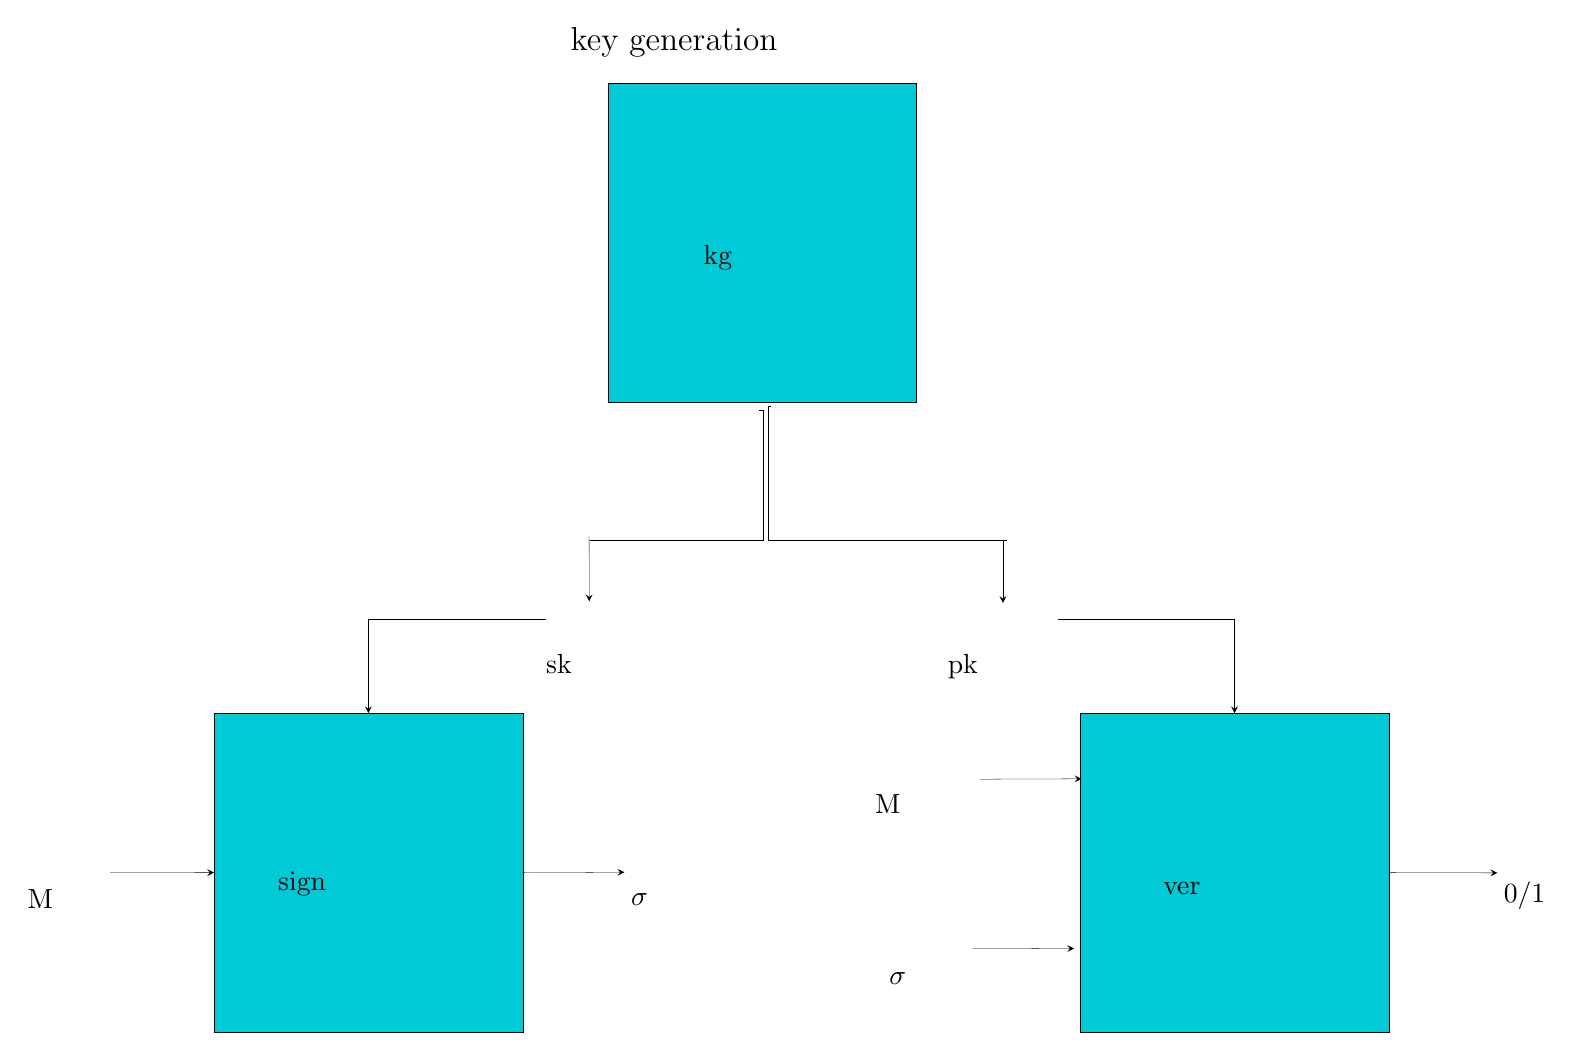
\begin{tikzpicture}[even odd rule]
\pgftransformxscale{1.000000}
\pgftransformyscale{-1.000000}
\definecolor{dialinecolor}{rgb}{0.000000, 0.000000, 0.000000}
\pgfsetstrokecolor{dialinecolor}
\pgfsetstrokeopacity{1.000000}
\definecolor{diafillcolor}{rgb}{1.000000, 1.000000, 1.000000}
\pgfsetfillcolor{diafillcolor}
\pgfsetfillopacity{1.000000}
\pgfsetlinewidth{0.100000\du}
\pgfsetdash{}{0pt}
\pgfsetbuttcap
\pgfsetmiterjoin
\pgfsetlinewidth{0.100000\du}
\pgfsetbuttcap
\pgfsetmiterjoin
\pgfsetdash{}{0pt}
{\pgfsetcornersarced{\pgfpoint{0.000000\du}{0.000000\du}}\definecolor{diafillcolor}{rgb}{0.000000, 0.792157, 0.839216}
\pgfsetfillcolor{diafillcolor}
\pgfsetfillopacity{1.000000}
\fill (7.782258\du,3.700000\du)--(7.782258\du,7.750000\du)--(11.701613\du,7.750000\du)--(11.701613\du,3.700000\du)--cycle;
}{\pgfsetcornersarced{\pgfpoint{0.000000\du}{0.000000\du}}\definecolor{dialinecolor}{rgb}{0.000000, 0.000000, 0.000000}
\pgfsetstrokecolor{dialinecolor}
\pgfsetstrokeopacity{1.000000}
\draw (7.782258\du,3.700000\du)--(7.782258\du,7.750000\du)--(11.701613\du,7.750000\du)--(11.701613\du,3.700000\du)--cycle;
}% setfont left to latex
\definecolor{dialinecolor}{rgb}{0.000000, 0.000000, 0.000000}
\pgfsetstrokecolor{dialinecolor}
\pgfsetstrokeopacity{1.000000}
\definecolor{diafillcolor}{rgb}{0.000000, 0.000000, 0.000000}
\pgfsetfillcolor{diafillcolor}
\pgfsetfillopacity{1.000000}
\node[anchor=base west,inner sep=0pt,outer sep=0pt,color=dialinecolor] at (9.000000\du,6.000000\du){kg};
\pgfsetlinewidth{0.100000\du}
\pgfsetdash{}{0pt}
\pgfsetbuttcap
\pgfsetmiterjoin
\pgfsetlinewidth{0.100000\du}
\pgfsetbuttcap
\pgfsetmiterjoin
\pgfsetdash{}{0pt}
{\pgfsetcornersarced{\pgfpoint{0.000000\du}{0.000000\du}}\definecolor{diafillcolor}{rgb}{0.000000, 0.792157, 0.839216}
\pgfsetfillcolor{diafillcolor}
\pgfsetfillopacity{1.000000}
\fill (2.782258\du,11.700000\du)--(2.782258\du,15.750000\du)--(6.701613\du,15.750000\du)--(6.701613\du,11.700000\du)--cycle;
}{\pgfsetcornersarced{\pgfpoint{0.000000\du}{0.000000\du}}\definecolor{dialinecolor}{rgb}{0.000000, 0.000000, 0.000000}
\pgfsetstrokecolor{dialinecolor}
\pgfsetstrokeopacity{1.000000}
\draw (2.782258\du,11.700000\du)--(2.782258\du,15.750000\du)--(6.701613\du,15.750000\du)--(6.701613\du,11.700000\du)--cycle;
}% setfont left to latex
\definecolor{dialinecolor}{rgb}{0.000000, 0.000000, 0.000000}
\pgfsetstrokecolor{dialinecolor}
\pgfsetstrokeopacity{1.000000}
\definecolor{diafillcolor}{rgb}{0.000000, 0.000000, 0.000000}
\pgfsetfillcolor{diafillcolor}
\pgfsetfillopacity{1.000000}
\node[anchor=base west,inner sep=0pt,outer sep=0pt,color=dialinecolor] at (3.596369\du,13.946183\du){sign};
\pgfsetlinewidth{0.100000\du}
\pgfsetdash{}{0pt}
\pgfsetbuttcap
\pgfsetmiterjoin
\pgfsetlinewidth{0.100000\du}
\pgfsetbuttcap
\pgfsetmiterjoin
\pgfsetdash{}{0pt}
{\pgfsetcornersarced{\pgfpoint{0.000000\du}{0.000000\du}}\definecolor{diafillcolor}{rgb}{0.000000, 0.792157, 0.839216}
\pgfsetfillcolor{diafillcolor}
\pgfsetfillopacity{1.000000}
\fill (13.782258\du,11.700000\du)--(13.782258\du,15.750000\du)--(17.701613\du,15.750000\du)--(17.701613\du,11.700000\du)--cycle;
}{\pgfsetcornersarced{\pgfpoint{0.000000\du}{0.000000\du}}\definecolor{dialinecolor}{rgb}{0.000000, 0.000000, 0.000000}
\pgfsetstrokecolor{dialinecolor}
\pgfsetstrokeopacity{1.000000}
\draw (13.782258\du,11.700000\du)--(13.782258\du,15.750000\du)--(17.701613\du,15.750000\du)--(17.701613\du,11.700000\du)--cycle;
}% setfont left to latex
\definecolor{dialinecolor}{rgb}{0.000000, 0.000000, 0.000000}
\pgfsetstrokecolor{dialinecolor}
\pgfsetstrokeopacity{1.000000}
\definecolor{diafillcolor}{rgb}{0.000000, 0.000000, 0.000000}
\pgfsetfillcolor{diafillcolor}
\pgfsetfillopacity{1.000000}
\node[anchor=base west,inner sep=0pt,outer sep=0pt,color=dialinecolor] at (14.838548\du,14.000000\du){ver};
% setfont left to latex
\definecolor{dialinecolor}{rgb}{0.000000, 0.000000, 0.000000}
\pgfsetstrokecolor{dialinecolor}
\pgfsetstrokeopacity{1.000000}
\definecolor{diafillcolor}{rgb}{0.000000, 0.000000, 0.000000}
\pgfsetfillcolor{diafillcolor}
\pgfsetfillopacity{1.000000}
\node[anchor=base west,inner sep=0pt,outer sep=0pt,color=dialinecolor] at (7.000000\du,11.200000\du){sk};
% setfont left to latex
\definecolor{dialinecolor}{rgb}{0.000000, 0.000000, 0.000000}
\pgfsetstrokecolor{dialinecolor}
\pgfsetstrokeopacity{1.000000}
\definecolor{diafillcolor}{rgb}{0.000000, 0.000000, 0.000000}
\pgfsetfillcolor{diafillcolor}
\pgfsetfillopacity{1.000000}
\node[anchor=base west,inner sep=0pt,outer sep=0pt,color=dialinecolor] at (12.100000\du,11.200000\du){pk};
% setfont left to latex
\definecolor{dialinecolor}{rgb}{0.000000, 0.000000, 0.000000}
\pgfsetstrokecolor{dialinecolor}
\pgfsetstrokeopacity{1.000000}
\definecolor{diafillcolor}{rgb}{0.000000, 0.000000, 0.000000}
\pgfsetfillcolor{diafillcolor}
\pgfsetfillopacity{1.000000}
\node[anchor=base west,inner sep=0pt,outer sep=0pt,color=dialinecolor] at (7.000000\du,10.000000\du){};
% setfont left to latex
\definecolor{dialinecolor}{rgb}{0.000000, 0.000000, 0.000000}
\pgfsetstrokecolor{dialinecolor}
\pgfsetstrokeopacity{1.000000}
\definecolor{diafillcolor}{rgb}{0.000000, 0.000000, 0.000000}
\pgfsetfillcolor{diafillcolor}
\pgfsetfillopacity{1.000000}
\node[anchor=base west,inner sep=0pt,outer sep=0pt,color=dialinecolor] at (11.178686\du,12.978978\du){M};
% setfont left to latex
\definecolor{dialinecolor}{rgb}{0.000000, 0.000000, 0.000000}
\pgfsetstrokecolor{dialinecolor}
\pgfsetstrokeopacity{1.000000}
\definecolor{diafillcolor}{rgb}{0.000000, 0.000000, 0.000000}
\pgfsetfillcolor{diafillcolor}
\pgfsetfillopacity{1.000000}
\node[anchor=base west,inner sep=0pt,outer sep=0pt,color=dialinecolor] at (0.414624\du,14.186366\du){M};
% setfont left to latex
\definecolor{dialinecolor}{rgb}{0.000000, 0.000000, 0.000000}
\pgfsetstrokecolor{dialinecolor}
\pgfsetstrokeopacity{1.000000}
\definecolor{diafillcolor}{rgb}{0.000000, 0.000000, 0.000000}
\pgfsetfillcolor{diafillcolor}
\pgfsetfillopacity{1.000000}
\node[anchor=base west,inner sep=0pt,outer sep=0pt,color=dialinecolor] at (11.357372\du,15.147153\du){$\sigma$};
% setfont left to latex
\definecolor{dialinecolor}{rgb}{0.000000, 0.000000, 0.000000}
\pgfsetstrokecolor{dialinecolor}
\pgfsetstrokeopacity{1.000000}
\definecolor{diafillcolor}{rgb}{0.000000, 0.000000, 0.000000}
\pgfsetfillcolor{diafillcolor}
\pgfsetfillopacity{1.000000}
\node[anchor=base west,inner sep=0pt,outer sep=0pt,color=dialinecolor] at (11.000000\du,15.000000\du){};
% setfont left to latex
\definecolor{dialinecolor}{rgb}{0.000000, 0.000000, 0.000000}
\pgfsetstrokecolor{dialinecolor}
\pgfsetstrokeopacity{1.000000}
\definecolor{diafillcolor}{rgb}{0.000000, 0.000000, 0.000000}
\pgfsetfillcolor{diafillcolor}
\pgfsetfillopacity{1.000000}
\node[anchor=base west,inner sep=0pt,outer sep=0pt,color=dialinecolor] at (8.078040\du,14.141215\du){$\sigma$};
% setfont left to latex
\definecolor{dialinecolor}{rgb}{0.000000, 0.000000, 0.000000}
\pgfsetstrokecolor{dialinecolor}
\pgfsetstrokeopacity{1.000000}
\definecolor{diafillcolor}{rgb}{0.000000, 0.000000, 0.000000}
\pgfsetfillcolor{diafillcolor}
\pgfsetfillopacity{1.000000}
\node[anchor=base west,inner sep=0pt,outer sep=0pt,color=dialinecolor] at (19.161144\du,14.098928\du){0/1};
\pgfsetlinewidth{0.100000\du}
\pgfsetdash{}{0pt}
\pgfsetmiterjoin
\pgfsetbuttcap
{
\definecolor{diafillcolor}{rgb}{0.000000, 0.000000, 0.000000}
\pgfsetfillcolor{diafillcolor}
\pgfsetfillopacity{1.000000}
% was here!!!
{\pgfsetcornersarced{\pgfpoint{0.000000\du}{0.000000\du}}\definecolor{dialinecolor}{rgb}{0.000000, 0.000000, 0.000000}
\pgfsetstrokecolor{dialinecolor}
\pgfsetstrokeopacity{1.000000}
\draw (9.703125\du,7.849999\du)--(9.761189\du,7.849999\du)--(9.761189\du,9.499999\du)--(7.561189\du,9.499999\du);
}}
\pgfsetlinewidth{0.100000\du}
\pgfsetdash{}{0pt}
\pgfsetmiterjoin
\pgfsetbuttcap
{
\definecolor{diafillcolor}{rgb}{0.000000, 0.000000, 0.000000}
\pgfsetfillcolor{diafillcolor}
\pgfsetfillopacity{1.000000}
% was here!!!
{\pgfsetcornersarced{\pgfpoint{0.000000\du}{0.000000\du}}\definecolor{dialinecolor}{rgb}{0.000000, 0.000000, 0.000000}
\pgfsetstrokecolor{dialinecolor}
\pgfsetstrokeopacity{1.000000}
\draw (9.850000\du,7.800000\du)--(9.813065\du,7.800000\du)--(9.813065\du,9.500000\du)--(12.850000\du,9.500000\du);
}}
\pgfsetlinewidth{0.100000\du}
\pgfsetdash{}{0pt}
\pgfsetbuttcap
{
\definecolor{diafillcolor}{rgb}{0.000000, 0.000000, 0.000000}
\pgfsetfillcolor{diafillcolor}
\pgfsetfillopacity{1.000000}
% was here!!!
\pgfsetarrowsend{stealth}
\definecolor{dialinecolor}{rgb}{0.000000, 0.000000, 0.000000}
\pgfsetstrokecolor{dialinecolor}
\pgfsetstrokeopacity{1.000000}
\draw (7.544724\du,9.449766\du)--(7.546334\du,10.279173\du);
}
\pgfsetlinewidth{0.100000\du}
\pgfsetdash{}{0pt}
\pgfsetbuttcap
{
\definecolor{diafillcolor}{rgb}{0.000000, 0.000000, 0.000000}
\pgfsetfillcolor{diafillcolor}
\pgfsetfillopacity{1.000000}
% was here!!!
\pgfsetarrowsend{stealth}
\definecolor{dialinecolor}{rgb}{0.000000, 0.000000, 0.000000}
\pgfsetstrokecolor{dialinecolor}
\pgfsetstrokeopacity{1.000000}
\draw (12.800000\du,9.500000\du)--(12.800000\du,10.300000\du);
}
\pgfsetlinewidth{0.100000\du}
\pgfsetdash{}{0pt}
\pgfsetmiterjoin
\pgfsetbuttcap
{
\definecolor{diafillcolor}{rgb}{0.000000, 0.000000, 0.000000}
\pgfsetfillcolor{diafillcolor}
\pgfsetfillopacity{1.000000}
% was here!!!
\pgfsetarrowsend{stealth}
{\pgfsetcornersarced{\pgfpoint{0.000000\du}{0.000000\du}}\definecolor{dialinecolor}{rgb}{0.000000, 0.000000, 0.000000}
\pgfsetstrokecolor{dialinecolor}
\pgfsetstrokeopacity{1.000000}
\draw (7.000000\du,10.500000\du)--(4.741935\du,10.500000\du)--(4.741935\du,11.700000\du);
}}
\pgfsetlinewidth{0.100000\du}
\pgfsetdash{}{0pt}
\pgfsetmiterjoin
\pgfsetbuttcap
{
\definecolor{diafillcolor}{rgb}{0.000000, 0.000000, 0.000000}
\pgfsetfillcolor{diafillcolor}
\pgfsetfillopacity{1.000000}
% was here!!!
\pgfsetarrowsend{stealth}
{\pgfsetcornersarced{\pgfpoint{0.000000\du}{0.000000\du}}\definecolor{dialinecolor}{rgb}{0.000000, 0.000000, 0.000000}
\pgfsetstrokecolor{dialinecolor}
\pgfsetstrokeopacity{1.000000}
\draw (13.500000\du,10.500000\du)--(15.741935\du,10.500000\du)--(15.741935\du,11.700000\du);
}}
\pgfsetlinewidth{0.100000\du}
\pgfsetdash{}{0pt}
\pgfsetbuttcap
{
\definecolor{diafillcolor}{rgb}{0.000000, 0.000000, 0.000000}
\pgfsetfillcolor{diafillcolor}
\pgfsetfillopacity{1.000000}
% was here!!!
\pgfsetarrowsend{stealth}
\definecolor{dialinecolor}{rgb}{0.000000, 0.000000, 0.000000}
\pgfsetstrokecolor{dialinecolor}
\pgfsetstrokeopacity{1.000000}
\draw (1.461460\du,13.724458\du)--(2.782258\du,13.725000\du);
}
\pgfsetlinewidth{0.100000\du}
\pgfsetdash{}{0pt}
\pgfsetbuttcap
{
\definecolor{diafillcolor}{rgb}{0.000000, 0.000000, 0.000000}
\pgfsetfillcolor{diafillcolor}
\pgfsetfillopacity{1.000000}
% was here!!!
\pgfsetarrowsend{stealth}
\definecolor{dialinecolor}{rgb}{0.000000, 0.000000, 0.000000}
\pgfsetstrokecolor{dialinecolor}
\pgfsetstrokeopacity{1.000000}
\draw (17.701613\du,13.725000\du)--(19.079325\du,13.728557\du);
}
\pgfsetlinewidth{0.100000\du}
\pgfsetdash{}{0pt}
\pgfsetbuttcap
{
\definecolor{diafillcolor}{rgb}{0.000000, 0.000000, 0.000000}
\pgfsetfillcolor{diafillcolor}
\pgfsetfillopacity{1.000000}
% was here!!!
\pgfsetarrowsend{stealth}
\definecolor{dialinecolor}{rgb}{0.000000, 0.000000, 0.000000}
\pgfsetstrokecolor{dialinecolor}
\pgfsetstrokeopacity{1.000000}
\draw (6.701613\du,13.725000\du)--(7.991503\du,13.720273\du);
}
\pgfsetlinewidth{0.100000\du}
\pgfsetdash{}{0pt}
\pgfsetbuttcap
{
\definecolor{diafillcolor}{rgb}{0.000000, 0.000000, 0.000000}
\pgfsetfillcolor{diafillcolor}
\pgfsetfillopacity{1.000000}
% was here!!!
\pgfsetarrowsend{stealth}
\definecolor{dialinecolor}{rgb}{0.000000, 0.000000, 0.000000}
\pgfsetstrokecolor{dialinecolor}
\pgfsetstrokeopacity{1.000000}
\draw (12.509534\du,12.538433\du)--(13.799424\du,12.533705\du);
}
\pgfsetlinewidth{0.100000\du}
\pgfsetdash{}{0pt}
\pgfsetbuttcap
{
\definecolor{diafillcolor}{rgb}{0.000000, 0.000000, 0.000000}
\pgfsetfillcolor{diafillcolor}
\pgfsetfillopacity{1.000000}
% was here!!!
\pgfsetarrowsend{stealth}
\definecolor{dialinecolor}{rgb}{0.000000, 0.000000, 0.000000}
\pgfsetstrokecolor{dialinecolor}
\pgfsetstrokeopacity{1.000000}
\draw (12.414935\du,14.693178\du)--(13.704826\du,14.688451\du);
}
% setfont left to latex
\definecolor{dialinecolor}{rgb}{0.000000, 0.000000, 0.000000}
\pgfsetstrokecolor{dialinecolor}
\pgfsetstrokeopacity{1.000000}
\definecolor{diafillcolor}{rgb}{0.000000, 0.000000, 0.000000}
\pgfsetfillcolor{diafillcolor}
\pgfsetfillopacity{1.000000}
\node[anchor=base west,inner sep=0pt,outer sep=0pt,color=dialinecolor] at (7.311227\du,3.287261\du){\large key generation};
\end{tikzpicture}

\normalsize}}

\bnm
  \AdvUFCMA{\DS}{\advA} = \Prob{\UFCMA_{\DS}^\advA\Rightarrow\true}
\enm

  \caption{Our desired asymmetric signature primitive allows for message authentication using a public key.  The security game is shown to the left, with the operation of the \texttt{kg}, \texttt{sign}, and \texttt{ver} primitives shown on the right.  $\sigma$ is referred to as the signature.  The sign operation is often randomized.  }
\label{fig:digsigvisual}
\end{figure}

Figure~\ref{fig:digsigvisual} shows the UF-CMA security game and a visual representation of the operation of our desired digital signature primitives.  An encryption key consists of a key generation routing, which generates a randomized secret and public key, and a signing routine that outputs a signature for a message given the secret key.

Formally, a digital signature scheme $\DS = (\kg,\sign,\ver)$ is a triple of
algorithms. Key generation is randomized and outputs a key pair $(\pk,\sk)$,
where $\pk$ is called the public or verification key and $\sk$ is called the secret or
signing key.
Signing takes as input a secret key $\sk$ and a message $M$ and outputs a
signature, usually denoted $\sigma$.
Verification takes as input a public key $\pk$, message $M$, and signature
$\sigma$ and outputs a
bit.

The advantage of an adversary against $\UFCMA_{\DS}$ security is defined as the probability it can generate a signature accepted by \texttt{ver} that was not generated by a signing oracle to which it has access.  Unlike in the message integrity $\UFCMA$ setting, we give the adversary access to the public key, as this key is public knowledge.  This implies the adversary can also run \texttt{ver} to check the validity of signatures.

We will now take show that one strawman plaintext RSA-based digital signature scheme fails to meet $\UFCMA_{\DS}$ security, then informally argue that another RSA-based scheme that is widely used in practice, PKCS v1.5, also fails to meet $\UFCMA_{\DS}$ security; the full proof is left as an exercise to the reader.  We then complete our analysis by proving $\UFCMA_{\DS}$ security for the ``full domain hash" RSA scheme.

\subsection{Straw-Man: Plaintext RSA}


\begin{figure}[h]
\centering
\fpage{.3}{
		\underline{$\kg$}\\
		Generate RSA (sk, pk) $((N, d), (N, e))$ \\
    Ret $((N,d), (N, e))$\\ \\
		\underline{$\sign((N, d), M)$}\\
    Ret $M^d\mod N$\\ \\
		\underline{$\ver((N, e), M, \sigma)$}\\
    Ret $\sigma^e\mod N = M$
}
\fpage{.25}{
		\underline{$\advA^{\SignOracle}(\pk=(N, e))$}\\
		$M^* \getsr Z^*_N$ \\
		$R \getsr Z^*_N$ \\
		$\sigma^* \gets \Sign(R^e M^*\mod N)$ \\
		Ret $(M^*, (\sigma^* R^{-1})\mod N)$
}
\bnm
  \AdvUFCMA{\DS}{\advA^\SignOracle} = \Prob{\UFCMA_{\DS}^{\advA^\SignOracle}\Rightarrow\true} \approx 1
\enm

  \caption{The plaintext RSA operation (left) uses the same key format and general structure as RSA encryption.  The adversary for this scheme (right) breaks $\UFCMA_{\DS}$ security with advantage of approximately 1.}
\label{fig:plaintextrsa}
\end{figure}

Figure~\ref{fig:plaintextrsa} shows a natural adaptation of plaintext (textbook) RSA to digital signatures.  The sign routine raises the message $M$ to the secret exponent $d$; for verification, the signature is raised to the public exponent $e$, taking advantage of the property that $m^{ed}\mod N=m\mod N$ (also used in RSA decryption to invert the RSA permutation without revealing the secret value $d$) for correctness.

However, the given adversary breaks $\UFCMA_{\DS}$ security with advantage of approximately 1, as we now argue.  Note that $\sigma^* = (R^e M^*)^d\mod N$ (by definition of sign) $ = (R^{ed} M^{*d})\mod N = (R^{ed}\mod N) (M^{*d}\mod N) = (R\mod N) (M^{*d}\mod N)$ (by RSA permutation) $ = \sigma$.

Note that the signature that our adversary returns for $M^*$ is $(\sigma R^{-1})\mod N$.  So, by the above, this is equal to $(R^{-1} ((R\mod N) (M^{*d}\mod N))\mod N = M^{*d}\mod N$, the exact signature generated by \texttt{sign} for $M^*$ by construction.

Note that our adversary generated a valid signature for $M^*$ making a single signing oracle query to $R^e M^*$.  Because $R$ is sampled at random from $\Z^*_N$, the probability that the adversary has queried the oracle on $M^* = $Pr$[R^e M^*=M^*] = \frac{1}{|\Z^*_N|}$.  Hence, our $A^\Sign$ wins the UF-CMA game with advantage $1 - \frac{1}{|\Z^*_N|} \approx 1$ for sufficiently large $N$.

Note that the above argument does not depend on a random choice of $M*$, and indeed applies to any $M^*$, which could be passed into our adversary as input.  This makes our attack a \emph{universal} forgery against RSA; that is, $\forall$ messages $M^*$, our adversary can provide a forged signature $\sigma^*$ without querying the real signature routine on $M^*$ with non-negligible advantage.  A weaker kind of forgery, \emph{existential forgery}, exists in a scheme if $\exists M^*$ such that an adversary can generate a forged signature $\sigma^*$ without querying the real signature routine on $M^*$ with non-negligible advantage.  Note that the existence of a universal forgery attack implies an existential forgery attack but not vice-versa, making universal forgery a stronger form of forgery than existential forgery.

\subsection{Insecurity in Practice: PKCSv1.5}


\begin{figure}[h]
\centering
\fpage{.25}{
		\underline{$\sign((N, d), M)$}\\
		$Y = 00 || 01 || FF^p || 00 || H(M)$
    Ret $Y^d\mod N$

}
\fpage{.45}{
		\underline{$\ver((N, e), M)$}\\
		$Y = \sigma^e\mod N$ \\
		Let $aa || bb || cc || dd || h = Y$ \\
		If $(aa \neq 00)$ or $(bb \neq 01)$ or $(cc \neq FF^p)$ or $(dd \neq 00)$: \\
		\myInd Ret error // Vulnerable to padding oracle attacks \\
		Ret $H(m) = h$

}

  \caption{The PKCS\#1 v1.5 signing construction uses a hash function to prevent the predictable algebraic manipulation of a message to which our plain-text straw man scheme is vulnerable.  In this case, let $N$ have $n$ bytes and the the output of $H$ have $m$ bytes; then, $p=n - m - 3$, providing a total output length of $n$ bytes.}
\label{fig:pkcs15sign}
\end{figure}



Figure~\ref{fig:pkcs15sign} shows a construction deployed in practice for RSA-based signing, PKCSv1.5.  In this scheme, the general structure of our plaintext RSA signing scheme is preserved, but the message is padded with additional data, and a hash of the message is included for exponentiation with the private RSA exponent rather than the full message.  This hash appears to protect against the form of attack we have seen above.

Intuitively, this makes malleability attacks like the form we have seen above more difficult; even if an adversary could use the techniques we show to generate a valid $\sigma$ for some $x=H(M')$ given a signature $\sigma^*$ for $H(M^*)$, they would be unlikely to generate a signature that verifies for a known message, as they would need to provide some $M'$ to a verification oracle along with $\sigma$ such that $H(M')=x$, inverting the hash function used for signing.  Use of a preimage resistant hash function therefore poses a barrier to an adversary's forgery attempts; they can generate a signature that is valid for \emph{some} message, without the ability to produce the message for which that signature is valid.  We formalize this intuition in the proof of Full-Domain RSA that follows.

The padding in the scheme also appears to provide additional protections: If, for example, an adversary changes bits in the padding section of signed values, the mangled padding should produce an error and fail to verify, further restricting the adversary's ability to produce valid signature values for some message without querying the signing oracle.  However, as previously explored in the notes, red flags should be raised about the use of padding in a context able to generate padding-specific errors; in fact, because the padding scheme is similar to that in RSA PKCS\#1 v1.5 encryption, the same attack is usable to extract key material in our signing scheme, violating $\UFCMA_{\DS}$ security.  The proof is left as an exercise to the reader.

We now move to a formal proof of $\UFCMA_{\DS}$ security for a hash-based RSA construction that \emph{does} provide such security.  We use a full domain hash to avoid such padding leakage issues, and to simplify our reasoning about the security of the scheme.

\subsection{A Secure Scheme: Full Domain RSA}


We now introduce the full domain hash (FDH) RSA scheme, denoted $\DS$.  Figure~\ref{fig:fulldomrsa} shows the operation of this scheme, a natural extension of plaintext RSA that simply hashes the message before exponentiating with a secret exponent.  Note that we model the hash function as a random oracle, which masks some subtle technical issues surrounding use of a hash with RSA; because $H(M)$ needs to be raised to the $d$ (mod $N$), $H(M)$ must output an element of the RSA group that can be exponentiated in the group.  So, the hash function used depends on the choice of $d$, complicating analysis.  We ignore these details in our consideration of the protocol, as they can be solved in practice by using a fixed output length hash that is indifferentiable from random oracles using existing hash functions, and mapping the output of the function to the relevant RSA group.

We now analyze the $\UFCMA_\DS$ security of our scheme.  We do so by reduction to RSA, showing specifically that for any adversary $A$ breaking the $\UFCMA_\DS$ of full domain RSA, we can construct an adversary $B$ for the RSA game with almost the same advantage.  Formally, let $q_h$ be the number of hash oracle queries performed by $A$ and $q_s$ be the number of signing oracle queries performed by $A$:

\begin{theorem*}
Let $\DS$ be the FDH scheme using $\RSAk$ and $\Horacle\Colon\msgspace\rightarrow\Z_N^*$ modeled as
a RO. Let $\advA$ be any $\UFCMA_\DS$-adversary making at most $q_h$ queries to
$\Horacle$ and $q_s$ queries to its signing oracle. 
Then we give an $\RSAk$-adversary $\advB$ such that
\bnm
    \AdvUFCMA{\DS}{\advA} \le (q_h + q_s + 1) \cdotsm\AdvOWF{\RSAk}{\advB}
\enm
Adversary~$\advB$ runs in time that of $\advA$ plus $\bigO(q_s+q_h)$. 
\end{theorem*}


\begin{proof}
To start we make some simplifying assumptions about $\advA$, and justify that these assumptions are without loss.

\textbf{Lemma 1} Let $A$ be any adversary that does not match our assumptions.  We will show that there exists some $A'$ such that $A'$ has the same advantage as $A$, and runs in at most $q_s+1$ additional oracle queries.  Let $M*$ be the message on which $A$ outputs a valid forgery, as in the game definition.

Our simplifications are as follows:
\begin{itemize}
	\item Whenever $A$ makes a query to $\SignOracle$ on a message $M$, it has previously made a query
$\Horacle(M)$.  If this assumption is not met, we transform $A$ to an equivalent $A'$ that queries $\Horacle(M)$ before $\Signoracle(M)$ for every query to the sign oracle, discarding the result.  Note that $A$ and $A'$ have identical output for all inputs, as our spurious oracle calls are discarded and do not affect the output subsequent calls to $\Horacle$ or $\Signoracle$ by inspection.  $A'$ runs in at most $q_s$ additional oracle queries by construction.
	\item $A$ always queries $\Horacle(M^*)$.  If not, at the end of executing $A$, $A'$ inserts and discards a synthetic query to $\Horacle(M^*)$. As in the above, spurious calls are disregarded and the advantage for $A, A'$ remains identical.  $A'$ runs in at most $1$ additional oracle query by construction.
	\item $A$ does not query $\Signoracle(M^*)$.  If instead $A$ does query $\Signoracle(M^*)$, we simply abort $A'$.  Note that if $A$ queries $\Signoracle(M^*)$, it succeeds with probability $0$, as by construction of the game $M*$ is in the set $\calM$ and has been signed by the oracle.  In this case, $A'$ fails (succeeds with probability $0$), meaning the advantage of $A'$ is exactly equal to that of $A$.  $A'$ makes one fewer oracle query than $A$ by construction.
	\item $A$ does not query $\Horacle$ or $\Signoracle$ twice on the same $M^*$.  If this is not the case, $A'$ can simply memoize all the deterministic calls to $\Horacle$ and $\Signoracle$, acting on the same oracle outputs as $A$ and thus yielding identical executions for all inputs without the need to repeat calls.  $A'$ makes fewer oracle queries than $A$ by construction.
\end{itemize}

So, we can consider only $A$ that meet our assumptions without loss of generality, as if such an $A$ exists, there exists an $A'$ that runs in at most $1+q_s$ additional $\Horacle$ oracle queries with the same advantage.  Lemma 1 holds.

\textbf{Toy example - No-message attack} Now, to build some intuition, let's first consider the case that $q_s = 0$, that is, 
we are arguing about unforgeability in a no-message attack where no legitimate signatures are produced by the signing oracle for the adversary.  Our key challenge is to construct such an adversary $B$ for RSA OWF, we must use an adversary for $\UFCMA_{\DS}$ as a black box.  Figure~\ref{fulldomaintoy} shows such an adversary, as well as the games required to prove security.  Our general proof will proceed by choosing a point $Y$ as the output of a simulated hash oracle, where $Y$ represents the point the adversary of an RSA OWF game needs to invert as a challenge.  Because our hash function is a random oracle, to recover the original signed message, our $\UFCMA_{\DS}$ adversary will need to invert the hash function on some queried point.  Specifically, they must do this on the point corresponding to the hash of $M^*$, the challenge for which they provide a valid signature; because our hash function is a random oracle, they must do this to get any information about the output of the hash function on $M^*$, required by construction to generate a valid signature (if no information about $H(M^*)$ is known, every possible output signature is equally likely by the RSA permutation's properties as a permutation).

Such an adversary can, however, query the hash oracle on multiple points, and it is not clear for which point to provide them with the OWF challenge $Y$.  
%Assume that $\advA$
%queries $\Horacle(M^*)$ where $M^*$ is the output message for its forgery. This
%is without loss. 
Our solution is to 
guess which random oracle query corresponds to the solution, and program its
output to be equal be the OWF challenge $Y$.  In more detail, we set our forgery
adversary $\advB$ to be as shown in Figure~\ref{fig:fulldomaintoy}.  Let $i^*$ be our guess for which index represents a query to $M^*$, and $i$ be the index of the next oracle query to be performed.
%Intuitively, to forge against FDH one needs to invert RSA on $\Horacle(M)$ for
%some $M$. Then we can build an inverter $\advB$ that works as follows. 

\begin{figure}
\centering
\fpage{.22}{
\underline{$\UFCMA_{\DS}$}\\
$((N,e),(N,d)) \getsr \kg$\\
$(M^*,\sigma^*) \getsr \advA^{\Horacle,\SignOracle}((N,e))$\\
If $M^* \in \calM$ then Ret $\false$\\
Ret $\left(\TabH[M^*] = (\sigma^*)^e \bmod N\right)$\medskip

\underline{$\Horacle(M)$}\\
If $\TabH[M] = \bot$ then\\
\myInd $\TabH[M] \getsr \Z_N^*$\\
Ret $\TabH[M]$\medskip

\underline{$\SignOracle(M)$}\\
$\calM \gets \calM \cup \{M\}$\\
$X \getsr \Horacle(M)$\\
Ret $X^d \bmod N$
}
\fpage{.22}{
\underline{$\G_0$ \;\;\; \fbox{$\G_1$}}\\
$((N,e),(N,d)) \getsr \kg$\\
$i^* \getsr [1,q]$\\
$i \gets 0$\\
$(M^*,\sigma^*) \getsr \advA^{\HashSim}((N,e))$\\
If $(M^* \ne M_{i^*})$ then \\
\myInd $\badtrue$\\
\myInd \fbox{Ret $\false$}\\
Ret $\left(\TabH[M^*] = (\sigma^*)^e \bmod N\right)$\medskip

\underline{$\HashSim(M)$}\\
$i \gets i+1$\\
$M_i \gets M$\\
If $i = i^*$ then\\
\myInd Ret $\TabH[M_i] \getsr \Z_N^*$\\
$\TabH[M_i] \getsr \Z_N^*$\\
Ret $\TabH[M_i]$
}
\fpage{.22}{
\underline{$\G_2$}\\
$((N,e),(N,d)) \getsr \kg$\\
$i^* \getsr [1,q]$\\
$i \gets 0$\\
$(M^*,\sigma^*) \getsr \advA^{\HashSim}((N,e))$\\
If $(M^* \ne M_{i^*})$ then \\
\myInd $\badtrue$\\
\myInd Ret $\false$\\
Ret $\left(\TabH[M^*] = (\sigma^*)^e \bmod N\right)$\medskip

\underline{$\HashSim(M)$}\\
$i \gets i+1$\\
$M_i \gets M$\\
If $i = i^*$ then\\
\myInd Ret $\TabH[M_i] \gets Y$\\
$\TabH[M_i] \getsr \Z_N^*$\\
Ret $\TabH[M_i]$
}
\fpage{.22}{
\underline{$\advB_{toy}((N,e),Y)$}\\
$(M^*,\sigma^*) \getsr \advA^{\HashSim}((N,e))$\\
Ret $\sigma^*$\medskip

\underline{$\HashSim(M)$}\\
If $i = i^*$ then\\
\myInd Ret $Y$\\
$X \getsr \Z_N^*$\\
Ret $X$
}
  \caption{Toy example of full-domain RSA hash signing with no signing queries.}
\label{fig:fulldomaintoy}
\end{figure}


Intuitively $\advB$ wins as long as $\advA$ wins and $i^*$ is the correct guess
of which hash query by $\advA$ corresponds to the winning $M^*$. (Recall that we
are assuming that $\advA$ always queries $\Horacle$ for the forgery message
$M^*$.) To analyze this, let game $\G_0$ be equal to $\UFCMA_{\DS}^\advA$ except
that it additionally includes a random choice of $i^* \getsr [1,q]$ and sets a
flag $\bad$ to true should $M^* \ne M_{i^*}$. Let
game $\G_1$ be the same as $\G_0$ except that  it chooses a random index $i^*
\getsr [1,q]$ and checks if $M^*$ is equal to the $i\thh$ random oracle
query. If not, it sets a flag $\bad$ to true and outputs $\false$, 
Otherwise it checks if $\advA$'s output is a winning forgery, outputing
$\true$ if so and $\false$ otherwise. Let $\good$ be the event that $\bad$ is
not set in game $\G_0$, and we let $\good$ be the same event for $\G_1$ (a
slight abuse of notation). Then we have that both games are
identical-until-$\bad$ and a variant of the fundamental lemma of game playing
says that:
\bnm
  \Prob{\G_0 \Rightarrow\true \land\good} = \Prob{\G_1\Rightarrow\true \land
  \good} \;.
\enm
Then using this, we have that:
\iffalse
\begin{align*}
\AdvOWF{\RSAk}{\advB_{toy}} 
%  &= \Prob{\G_0\Rightarrow\true} (1)
  &\ge \Prob{\G_0\Rightarrow\true\land\good} (2)\\
  &= \Prob{\G_1\Rightarrow\true\land\good} (3)\\
  &= \Prob{\G_1\Rightarrow\true}\cdot\Prob{\good} (4)\\
  &= \AdvUFCMA{\DS}{\advA}\cdotsm\frac{1}{q_h} (5)
\end{align*}
\fi

\begin{align*}
\AdvOWF{\RSAk}{\advB_{toy}} 
  &= \Prob{\G_2\Rightarrow\true} (1) \\
  &= \Prob{\G_1\Rightarrow\true} (2)
  \ge \Prob{\G_1\Rightarrow\true\land\good} (3)\\
  &= \Prob{\G_0\Rightarrow\true\land\good} (4)
  = \Prob{\G_0\Rightarrow\true}\cdot\Prob{\good} (5)\\
  &= \AdvUFCMA{\DS}{\advA}\cdotsm\frac{1}{q} (6)
\end{align*}


$(1)$ follows because $\G_0$ outputs \texttt{true} iff $\TabH[M^*] = (\sigma^*)^e \bmod N$.  Note that $\TabH[M^*] = Y$ (because $\G_0$ outputs false if $M_{i^*}\neq M^*$, and by construction of the hash oracle).  So, $Y=(\sigma^*)^e \bmod N$ for B's challenge in the OWF game, and $B$ outputs $(\sigma^*)$, winning the OWF game.

$(2)$ follows because $G_2, G_1$ differ only in the output of $\TabH[M^{M^*}]$ (as above, in both, either game returning true implies $M_{i^*} = M^*$).  But, in one case, a point sampled from $\calZ_N$ is returned, and in another, $Y$ is returned, which is a point sampled from $\calZ_N$ by definition of the challenge provided $B$ in the OWF game.  It is thus impossible for this difference in identically distributed random choice to affect the operation of $A$.

$(3)$ follows from basic probability, and $(4)$ follows from our variant of the fundamental lemma of game playing, above.  $(5)$ follows as the probability that the good flag is set in $G_1$ is exactly equal to the probability that $M^* = M_{i^*}$, which is by definition the probability that the $i^*$th query of $q_h$ total queries to the hash oracle has as input $M^*$.  Because $i$ is independently uniformly sampled, this probability is equal for every choice of $i$, independent of all other values. $(6)$ follows as Lemma 1 states that $M^*$ will be exactly one of the queries to the hash oracle (in this case equal to the number of total queries, $q$, as $q_s=0$), making this probability exactly equal to $\frac{1}{q}$.  Note that concretely here, $q=q_h+1$ by Lemma 1.

\textbf{Generalization of toy example to full proof}  We now must do a generalization of the above to cases where $q_s \geq 1$, that is, our black-box $\UFCMA_\DS$ adversary makes at least one signing query.  In these cases, we face a substantive challenge: because the hash function in our full domain RSA construction is used by the signing routine, it is not the case that sign function outputs are independent of the outputs of our hash function.  We therefore cannot simply return random points for both the sign and hash function, as this breaks the structure of signatures; for example, any adversary that runs \texttt{ver} on outputs of \texttt{sign} would receive outputs of $1$ with a valid signature and hash function, and $0$ if we return random points, altering its execution and therefore output with overwhelming probability.

We therefore must program the signature oracle to return points which constitute valid signatures for points on which the hash oracle has already been queried (by Lemma 1, we can assume this is always the case).  So, as desired, we have that $\AdvOWF{\RSAk}{\advB_{toy}} \ge \AdvUFCMA{\DS}{\advA}\cdotsm\frac{1}{q}$, completing the proof.



\begin{figure}
\centering
\fpage{.30}{
\underline{$\advB((N,e),Y)$}\\
$i^* \getsr [1,q]$\\
$i \gets 0$\\
$(M^*,\sigma^*) \getsr \advA^{\HashSim,\SignSim}((N,e))$\\
If $(M^* \ne M_{i^*})$ then $X' \getsr \Z_N^*$\\
Else $X' \gets \sigma^*$\\
Ret $X'$\medskip

\underline{$\HashSim(M)$}\\
$i \gets i+1$\\
$M_i \gets M$\\
If $i = i^*$ then\\
\myInd Ret $Y$\\
$\sigma_i \getsr \Z_N^*$\\
$\TabH[M_i] \gets (\sigma_i)^e \bmod N$\\
Ret $\TabH[M_i]$\medskip

\underline{$\SignSim(M)$}\\
Let $i$ be s.t.~$M_i = M$\\
If $i = i^*$ then\\
\myInd Ret $\sigma \getsr \Z_N^*$\\
Ret $\sigma_i$
}
\fpage{.30}{
\underline{$\G_0$}\\
$((N,e),(N,d) \getsr \kg$\\
$X \getsr \Z_N^*$\\
$Y \gets X^e \bmod N$\\
$i^* \getsr [1,q]$\\
$i \gets 0$\\
$(M^*,\sigma^*) \getsr \advA^{\HashSim,\SignSim}((N,e))$\\
If $(M^* \ne M_{i^*})$ then \\
\myInd $\badtrue$\\
\myInd $X' \getsr \Z_N^*$\\
$X' \gets \sigma^*$\\
Ret $(X = X')$\medskip

\underline{$\HashSim(M)$}\\
$i \gets i+1$\\
$M_i \gets M$\\
If $i = i^*$ then\\
\myInd Ret $Y$\\
$\sigma_i \getsr \Z_N^*$\\
$\TabH[M_i] \gets (\sigma_i)^e \bmod N$\\
Ret $\TabH[M_i]$\medskip

\underline{$\SignSim(M)$}\\
Let $i$ be s.t.~$M_i = M$\\
If $i = i^*$ then\\
\myInd $\badtrue$\\
\myInd Ret $\sigma \getsr \Z_N^*$\\
Ret $\sigma_i$
}
\fpage{.30}{
\underline{$\G_1$}\\
$((N,e),(N,d) \getsr \kg$\\
$X \getsr \Z_N^*$\\
$Y \gets X^e \bmod N$\\
$i^* \getsr [1,q]$\\
$i \gets 0$\\
$(M^*,\sigma^*) \getsr \advA^{\HashSim,\SignSim}((N,e))$\\
If $(M^* \ne M_{i^*})$ then \\
\myInd $\badtrue$\\
\myInd $X' \gets \sigma^*$\\
$X' \gets \sigma^*$\\
Ret $(X = X')$\medskip

\underline{$\HashSim(M)$}\\
$i \gets i+1$\\
$M_i \gets M$\\
If $i = i^*$ then\\
\myInd Ret $Y$\\
$\sigma_i \getsr \Z_N^*$\\
$\TabH[M_i] \gets (\sigma_i)^e \bmod N$\\
Ret $\TabH[M_i]$\medskip

\underline{$\SignSim(M)$}\\
Let $i$ be s.t.~$M_i = M$\\
If $i = i^*$ then\\
\myInd $\badtrue$\\
\myInd Ret $\sigma \gets X$\\
Ret $\sigma_i$
}


\begin{align*}
  \AdvUFCMA{\DS}{\advA} &= \Prob{\G_1\Rightarrow\true}\\
      &\le \Prob{\G_0\Rightarrow\true} + \Prob{\bad_0}\\
      &= \AdvOWF{\RSAk}{\advB} + \Prob{\bad_0}
\end{align*}

  \caption{Extension of our toy example to a full proof, simulating signing oracle points.}
\label{fig:fulldomainsignproof}
\end{figure}

\textbf{TODO Lucy; describe/check Figure~\ref{fig:fulldomainsignproof} and merge with the toy proof; the proof should be mainly unchanged.}

\end{proof}


\subsection{Questions}

\begin{enumerate}
\item You are the hacker that has discovered the \texttt{goto fail} vulnerability!  Consider a server $S$ and a client $C$ performing the key exchange in Figure~\ref{fig:mitmdiffie}, where the client certificate check unconditionally returns true.  Provide a concrete man-in-the-middle attack on the resulting protocol, and argue that the protocol completes successfully on both the server and client side while leaking messages to an adversary; if this is not possible, provide clear intuition for why not.
\item Our full-domain hash proof of RSA involves choosing a random point in the hashing oracle to puncture and return our desired RSA point $Y$.  What if instead of selecting such a point randomly, the first call to the oracle was used?  Does the argument in the proof hold?  Provide a reason the proof holds or counterexample of an adversary for which the proof fails to hold.
\item Figure~\ref{fig:pkcs15sign} shows the PKCS\#1 v1.5 RSA-based signing scheme.  Argue that the scheme is vulnerable to padding oracle attacks.
\end{enumerate}